\documentclass{beamer}
\usepackage[spanish]{babel}
\usepackage[utf8]{inputenc}
\usepackage{listings}
\usepackage{color}
\usepackage[T1]{fontenc}
\usepackage[T1]{fontenc}
\usetheme[pageofpages=of,% String used between the current page and the
          bullet=circle,% Use circles instead of squares for bullets.
          titleline=true,% Show a line below the frame title.
          alternativetitlepage=true,% Use the fancy title page.
          ]{Torino}

\graphicspath{{images/}}
%%%%%%%%%%%%%%%%%%%%%%%%%%%%%%%%%%%%%%%%%%%%%%%%%%%%%%%%%%%%%%%%%%%%%%%%%%
\title{Introducci\'on a Linux con OpenSuse}
\author{Jennifer Maldonado}
\date{\today}

\begin{document}
%%%%%%%%%%%%%%%%%%%%%%%%%%%%%%%%%%%%%%%%%%%%%%%%%%%%%%%%%%%%%%%%%%%%%%%%%%
\begin{frame}
\titlepage
\end{frame}
%%%%%%%%%%%%%%%%%%%%%%%%%%%%%%%%%%%%%%%%%%%%%%%%%%%%%%%%%%%%%%%%%%%%%%%%%%
\setcounter{tocdepth}{1}
\begin{frame}[allowframebreaks]
\frametitle{\'Indice}
\tableofcontents
\end{frame}
%%%%%%%%%%%%%%%%%%%%%%%%%%%%%%%%%%%%%%%%%%%%%%%%%%%%%%%%%%%%%%%%%%%%%%%%%%
\section{El Filesystem Hierarchy Standard}
\subsection{Estructura del \'arbol de directorios}
\begin{frame}
\setcounter{tocdepth}{3}
\tableofcontents[currentsection]
\frametitle{El Sistema de Archivos}
\end{frame} 
%%%%%%%%%%%%%%%%%%%%%%%%%%%%%%%%%%%%%%%%%%%%%%%%%%%%%%%%%%%%%%%%%%%%%%%%%%
\begin{frame}
\frametitle{El Sistema de Archivos}
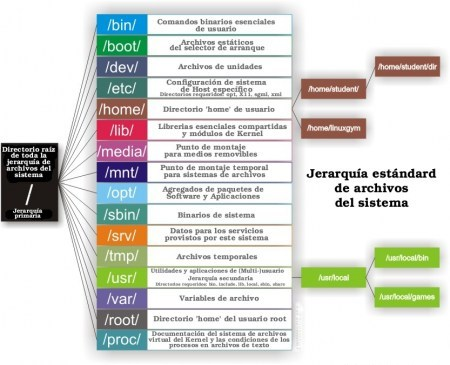
\includegraphics[height=0.8\textheight]{fhs-esp.jpg} \hspace*{7.3cm}
\end{frame} 
%%%%%%%%%%%%%%%%%%%%%%%%%%%%%%%%%%%%%%%%%%%%%%%%%%%%%%%%%%%%%%%%%%%%%%%%%%
\section{Instalaci\'on del sistema Opensuse}
\subsection{Configuraci\'on general}
\begin{frame}
\frametitle{La Instalaci\'on}
\tableofcontents[currentsection]
\end{frame} 
%%%%%%%%%%%%%%%%%%%%%%%%%%%%%%%%%%%%%%%%%%%%%%%%%%%%%%%%%%%%%%%%%%%%%%%%%%
\begin{frame}
\frametitle{La Instalaci\'on}
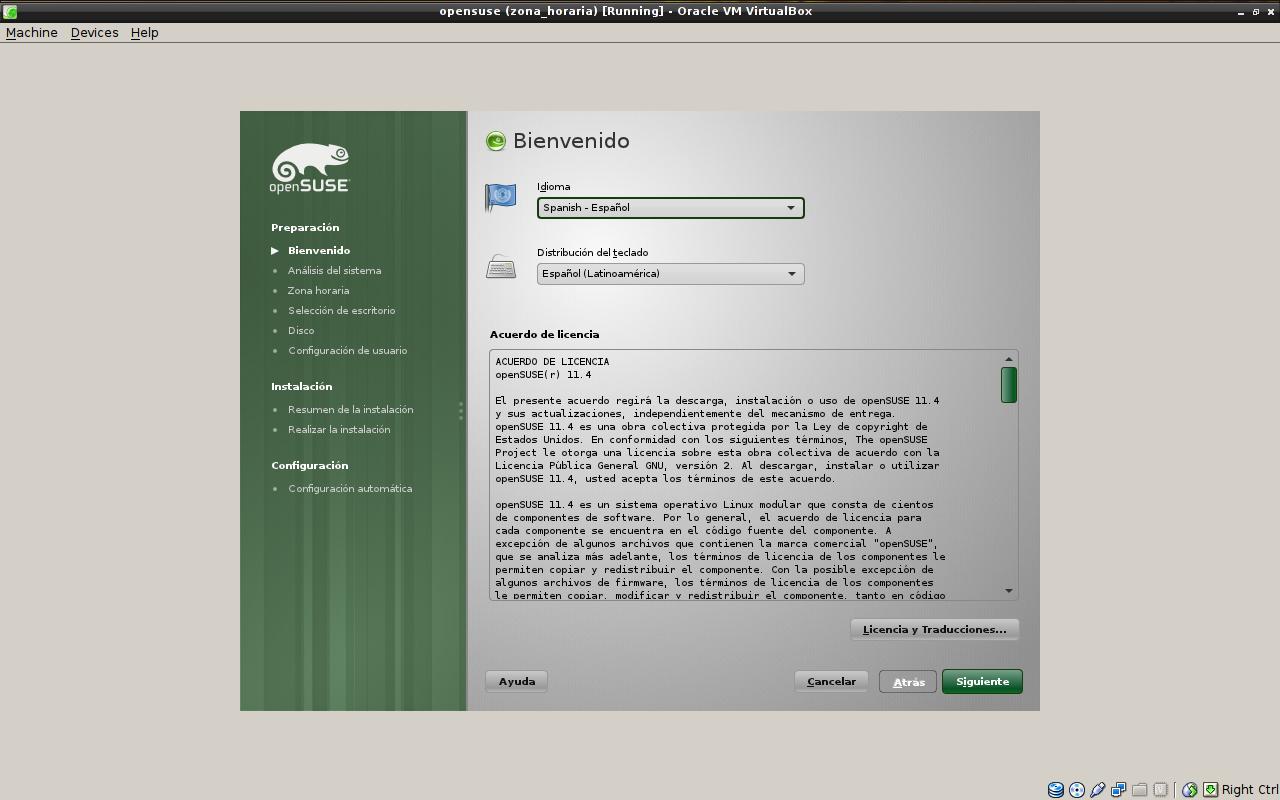
\includegraphics[height=0.8\textheight]{0_.png} \hspace*{7.3cm}
\end{frame} 
%%%%%%%%%%%%%%%%%%%%%%%%%%%%%%%%%%%%%%%%%%%%%%%%%%%%%%%%%%%%%%%%%%%%%%%%%%
\begin{frame}
\frametitle{La Instalaci\'on}
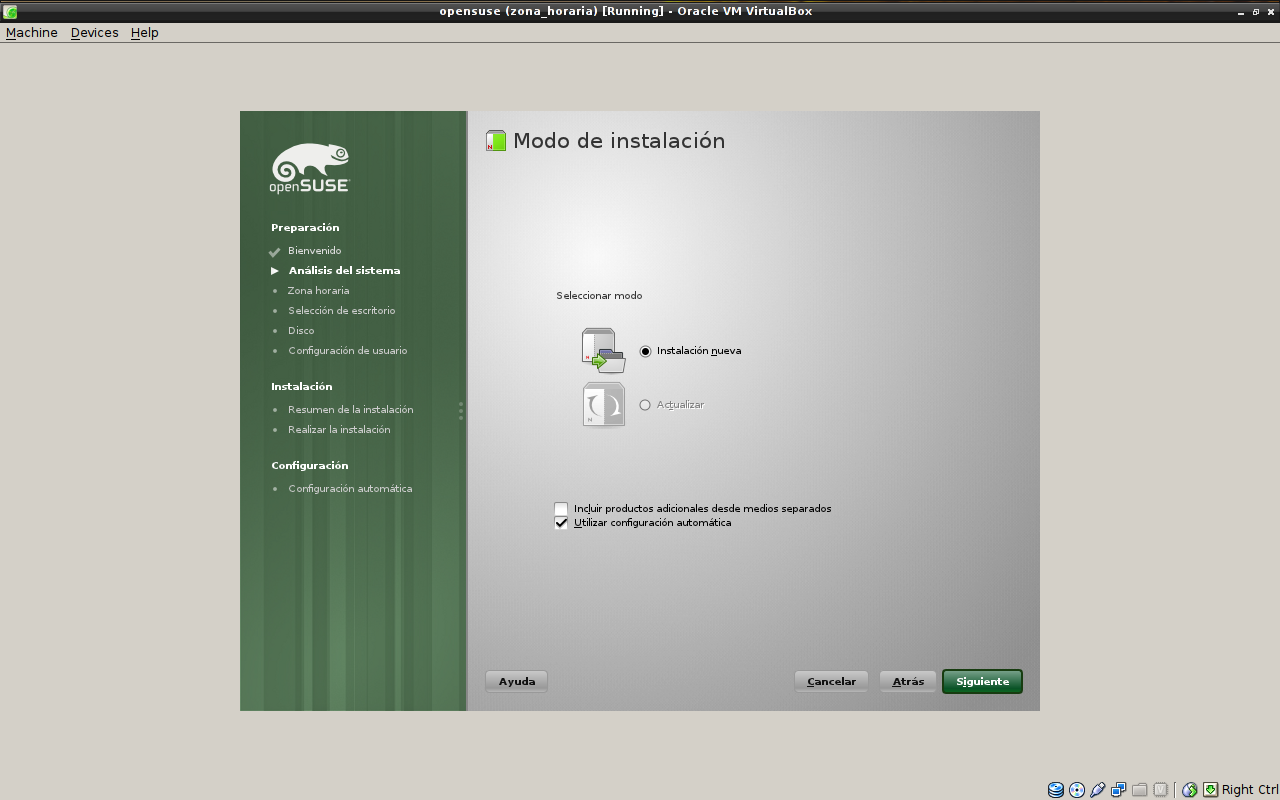
\includegraphics[height=0.8\textheight]{1_.png} \hspace*{7.3cm}
\end{frame} 
%%%%%%%%%%%%%%%%%%%%%%%%%%%%%%%%%%%%%%%%%%%%%%%%%%%%%%%%%%%%%%%%%%%%%%%%%%
\begin{frame}
\frametitle{La Instalaci\'on}
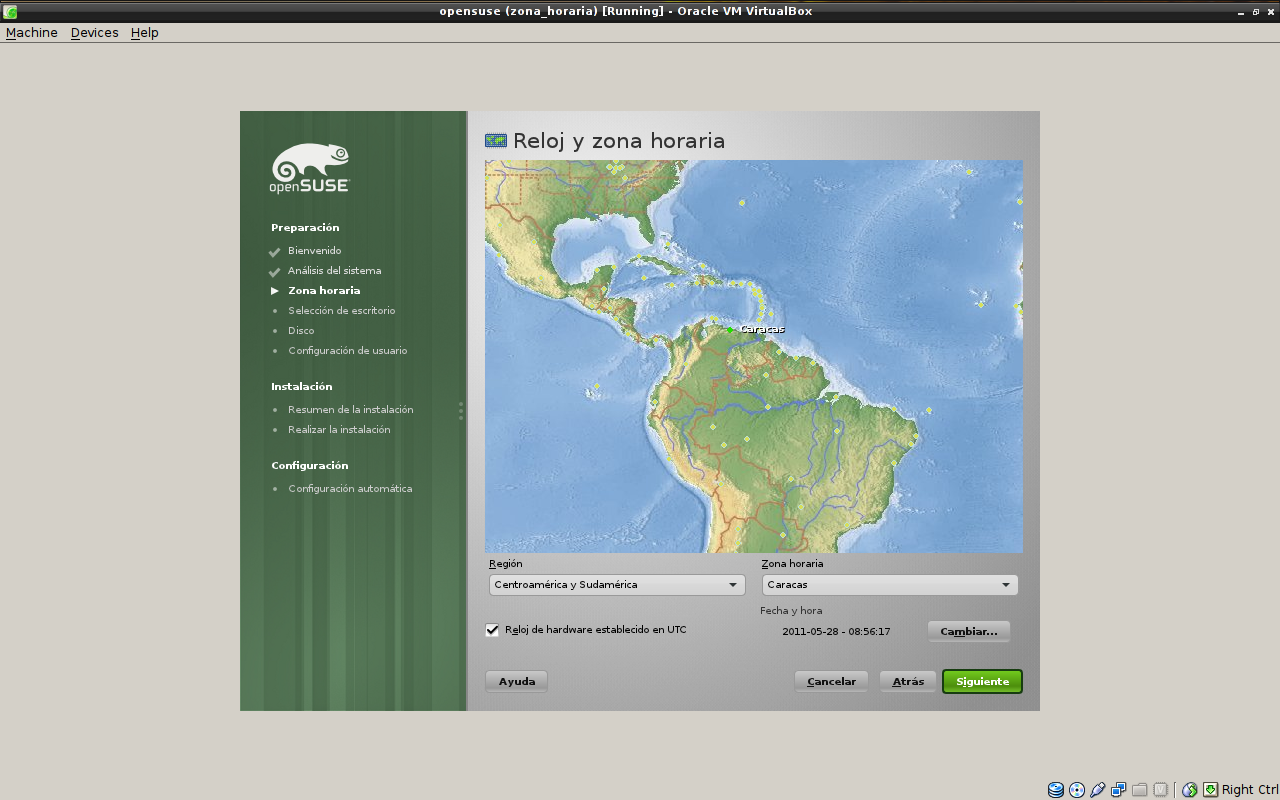
\includegraphics[height=0.8\textheight]{2.png} \hspace*{7.3cm}
\end{frame} 
%%%%%%%%%%%%%%%%%%%%%%%%%%%%%%%%%%%%%%%%%%%%%%%%%%%%%%%%%%%%%%%%%%%%%%%%%%
\begin{frame}
\frametitle{La Instalaci\'on}
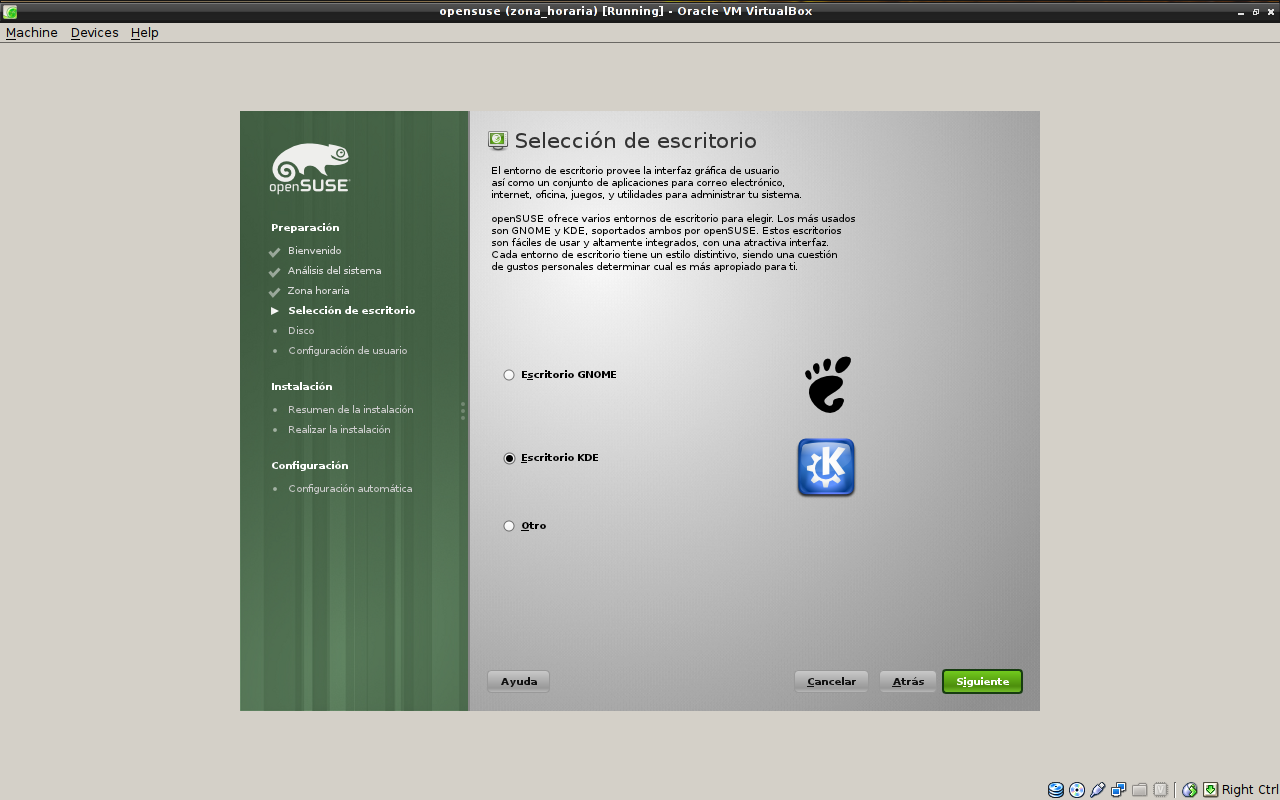
\includegraphics[height=0.8\textheight]{3_.png} \hspace*{7.3cm}
\end{frame} 
%%%%%%%%%%%%%%%%%%%%%%%%%%%%%%%%%%%%%%%%%%%%%%%%%%%%%%%%%%%%%%%%%%%%%%%%%%
\begin{frame}
\frametitle{La Instalaci\'on}
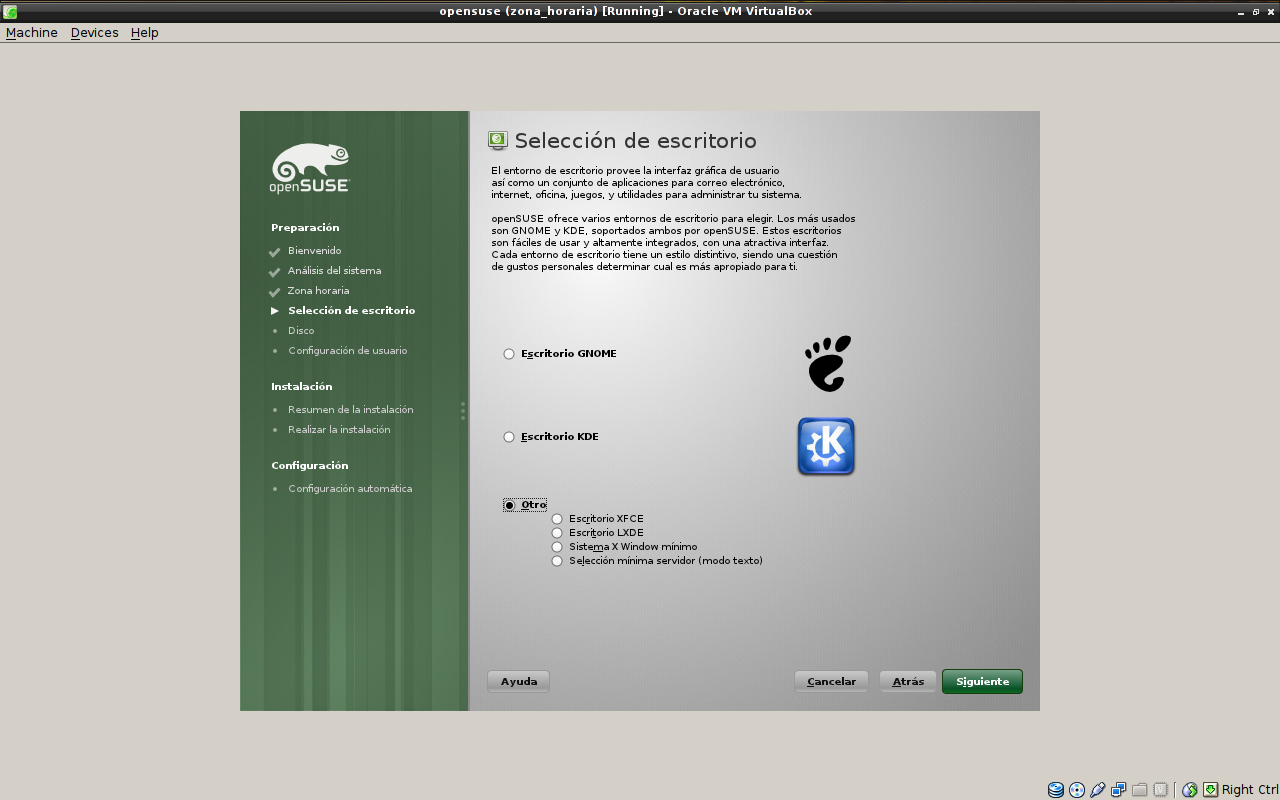
\includegraphics[height=0.8\textheight]{4_.png} \hspace*{7.3cm}
\end{frame} 
%%%%%%%%%%%%%%%%%%%%%%%%%%%%%%%%%%%%%%%%%%%%%%%%%%%%%%%%%%%%%%%%%%%%%%%%%%
\begin{frame}
\frametitle{La Instalaci\'on}
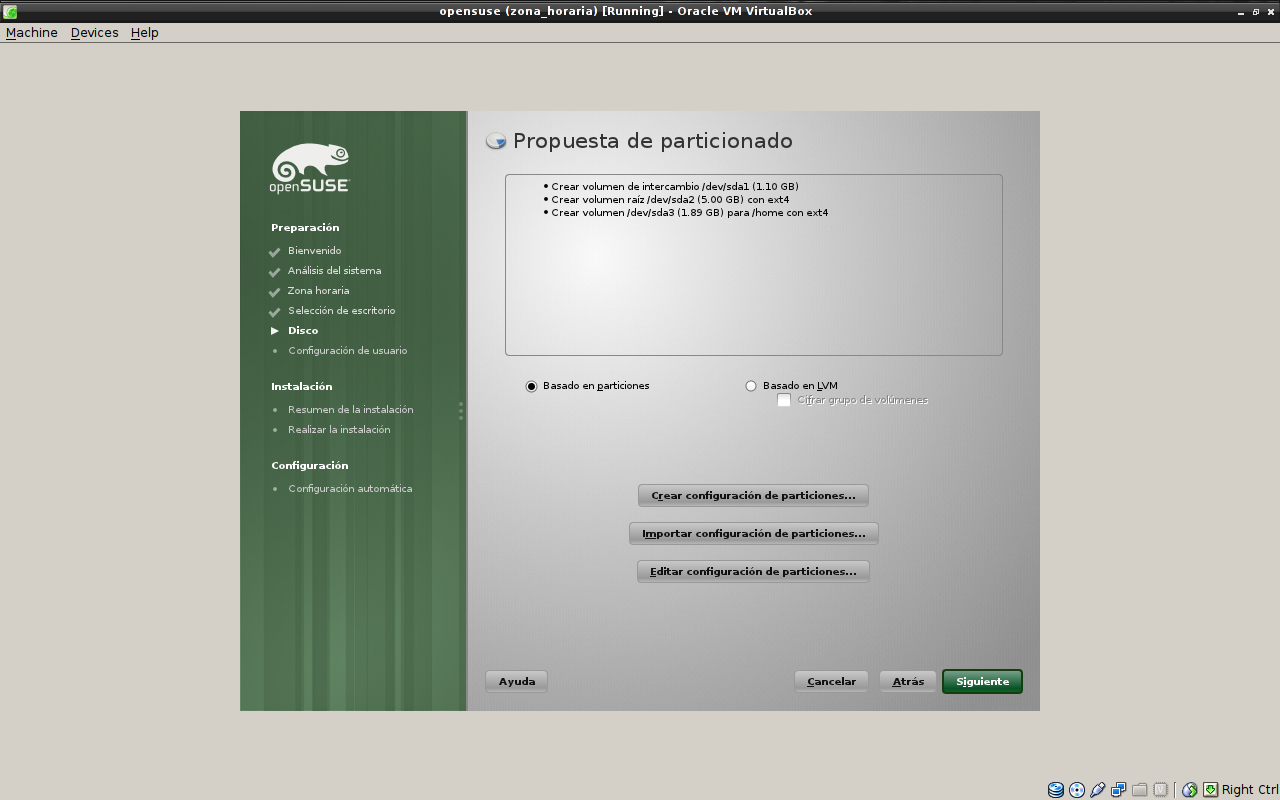
\includegraphics[height=0.8\textheight]{5_.png} \hspace*{7.3cm}
\end{frame} 
%%%%%%%%%%%%%%%%%%%%%%%%%%%%%%%%%%%%%%%%%%%%%%%%%%%%%%%%%%%%%%%%%%%%%%%%%%
\subsection{Particionamiento}
\begin{frame}
\frametitle{La Instalaci\'on}
\tableofcontents[currentsubsection]
\end{frame} 
%%%%%%%%%%%%%%%%%%%%%%%%%%%%%%%%%%%%%%%%%%%%%%%%%%%%%%%%%%%%%%%%%%%%%%%%%%

\begin{frame}
\frametitle{La Instalaci\'on}
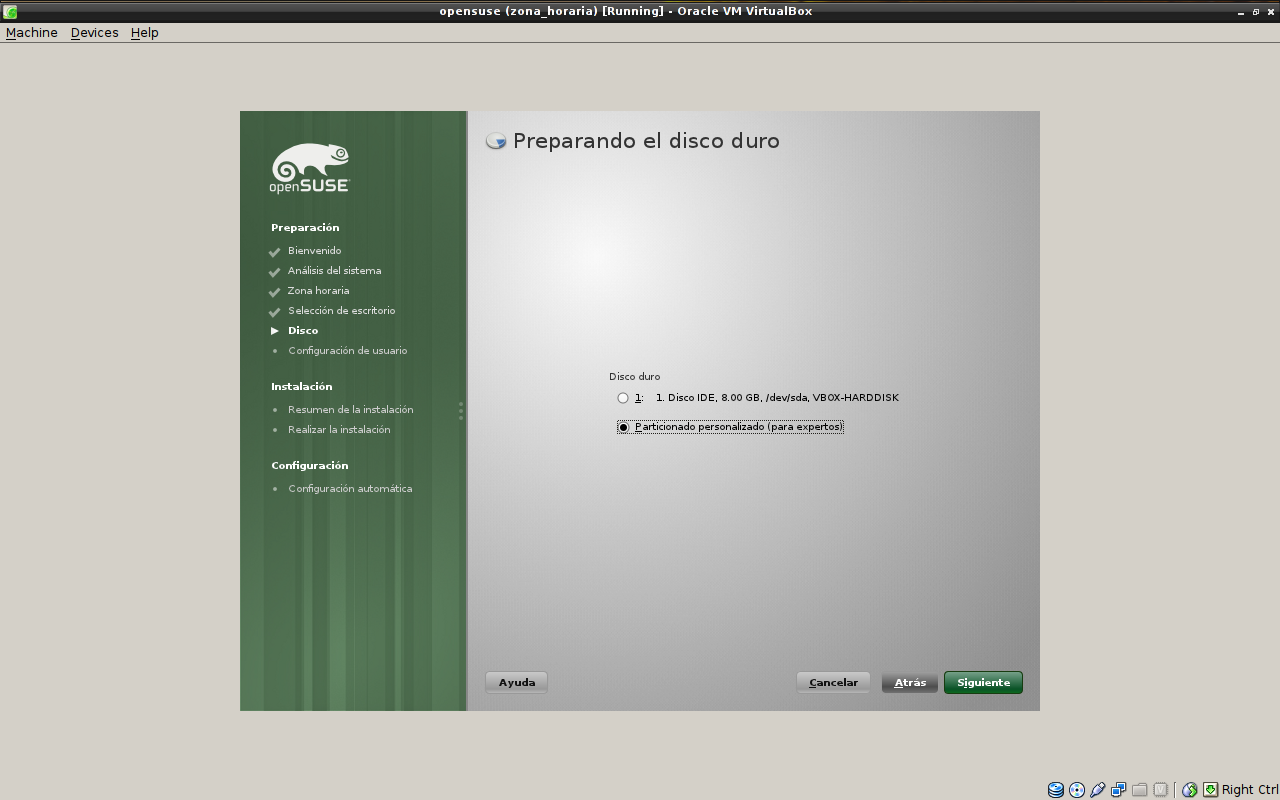
\includegraphics[height=0.8\textheight]{6.png} \hspace*{7.3cm}
\end{frame} 
%%%%%%%%%%%%%%%%%%%%%%%%%%%%%%%%%%%%%%%%%%%%%%%%%%%%%%%%%%%%%%%%%%%%%%%%%%

\begin{frame}
\frametitle{La Instalaci\'on}
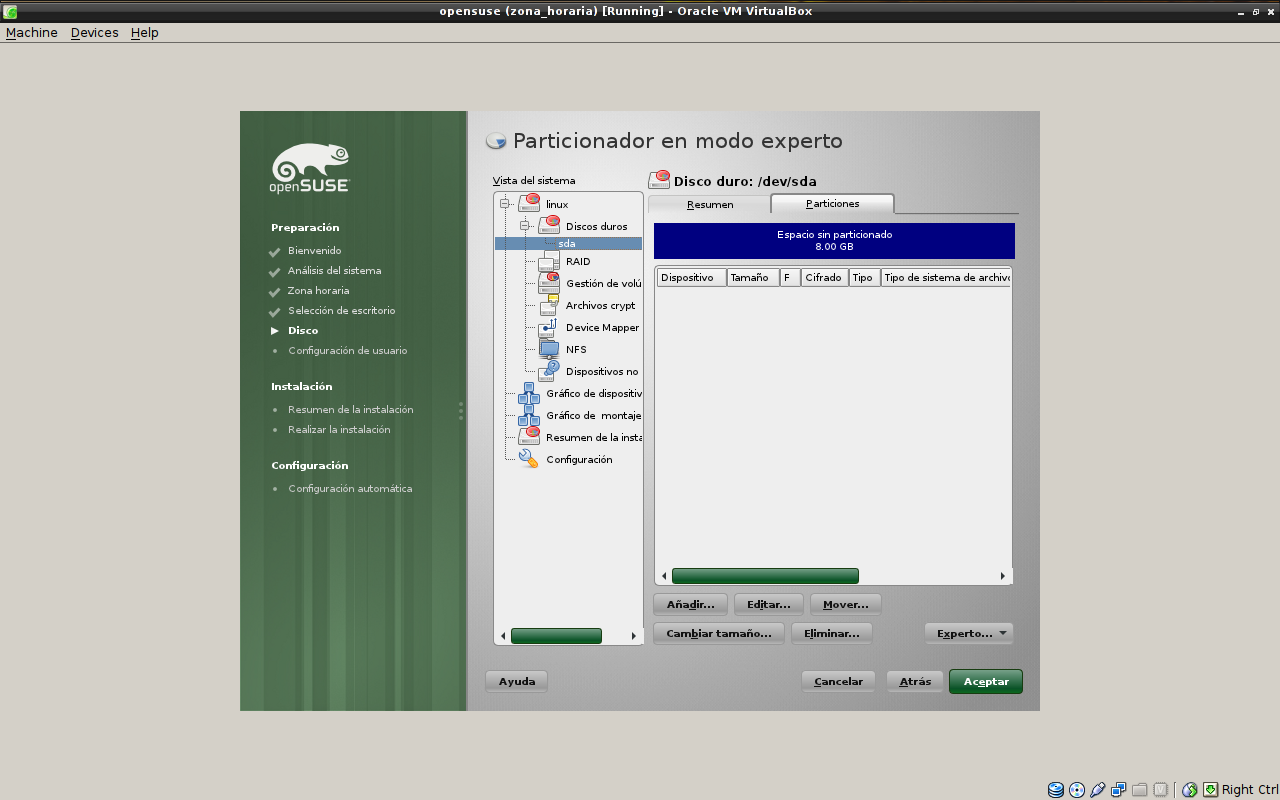
\includegraphics[height=0.8\textheight]{7.png} \hspace*{7.3cm}
\end{frame} 
%%%%%%%%%%%%%%%%%%%%%%%%%%%%%%%%%%%%%%%%%%%%%%%%%%%%%%%%%%%%%%%%%%%%%%%%%%

\begin{frame}
\frametitle{La Instalaci\'on}
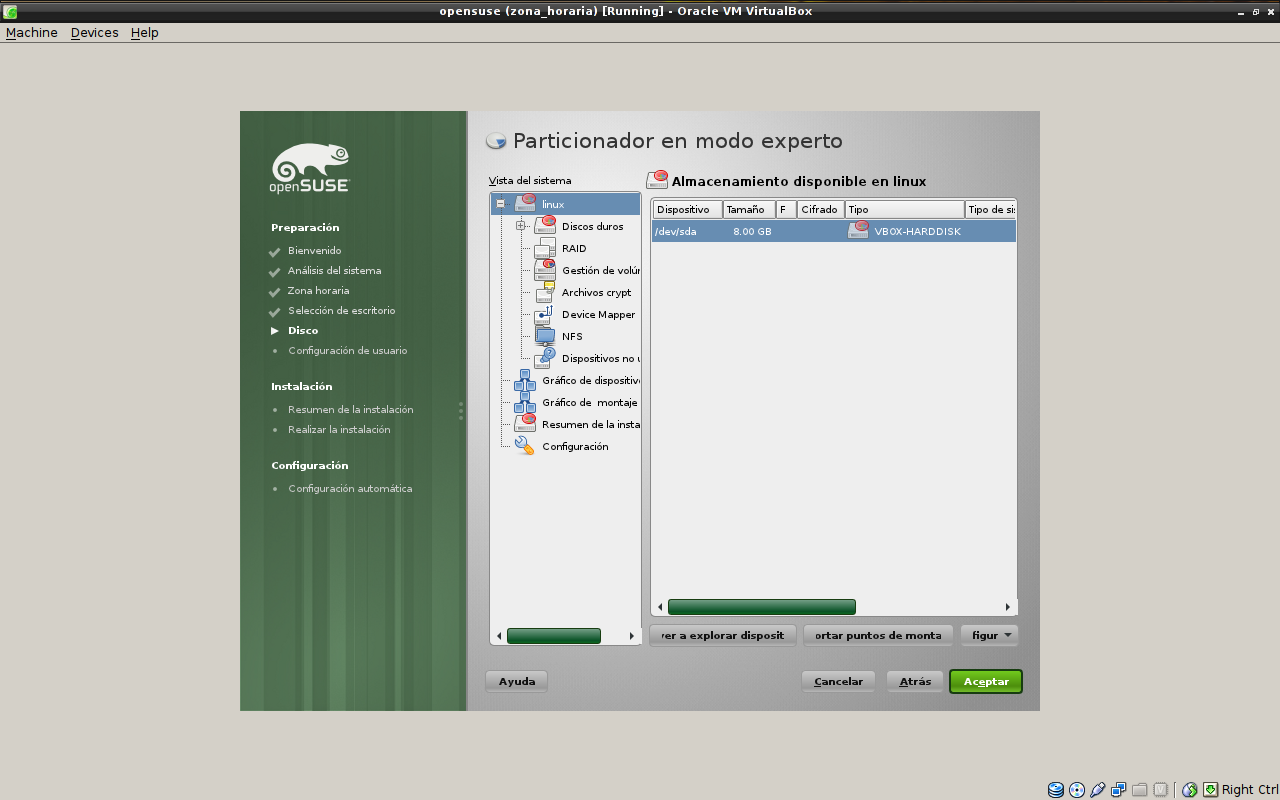
\includegraphics[height=0.8\textheight]{7_.png} \hspace*{7.3cm}
\end{frame} 
%%%%%%%%%%%%%%%%%%%%%%%%%%%%%%%%%%%%%%%%%%%%%%%%%%%%%%%%%%%%%%%%%%%%%%%%%%

\begin{frame}
\frametitle{La Instalaci\'on}
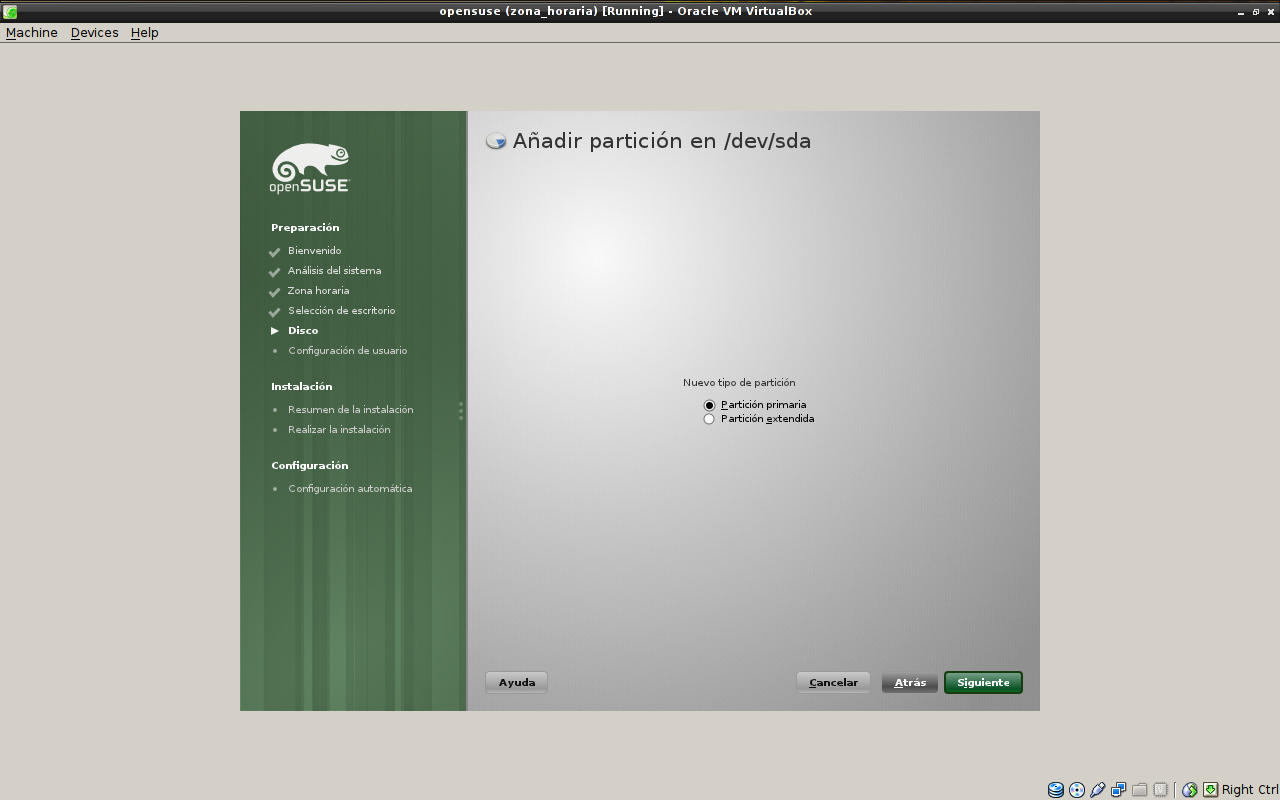
\includegraphics[height=0.8\textheight]{8.png} \hspace*{7.3cm}
\end{frame} 
%%%%%%%%%%%%%%%%%%%%%%%%%%%%%%%%%%%%%%%%%%%%%%%%%%%%%%%%%%%%%%%%%%%%%%%%%%

\begin{frame}
\frametitle{La Instalaci\'on}
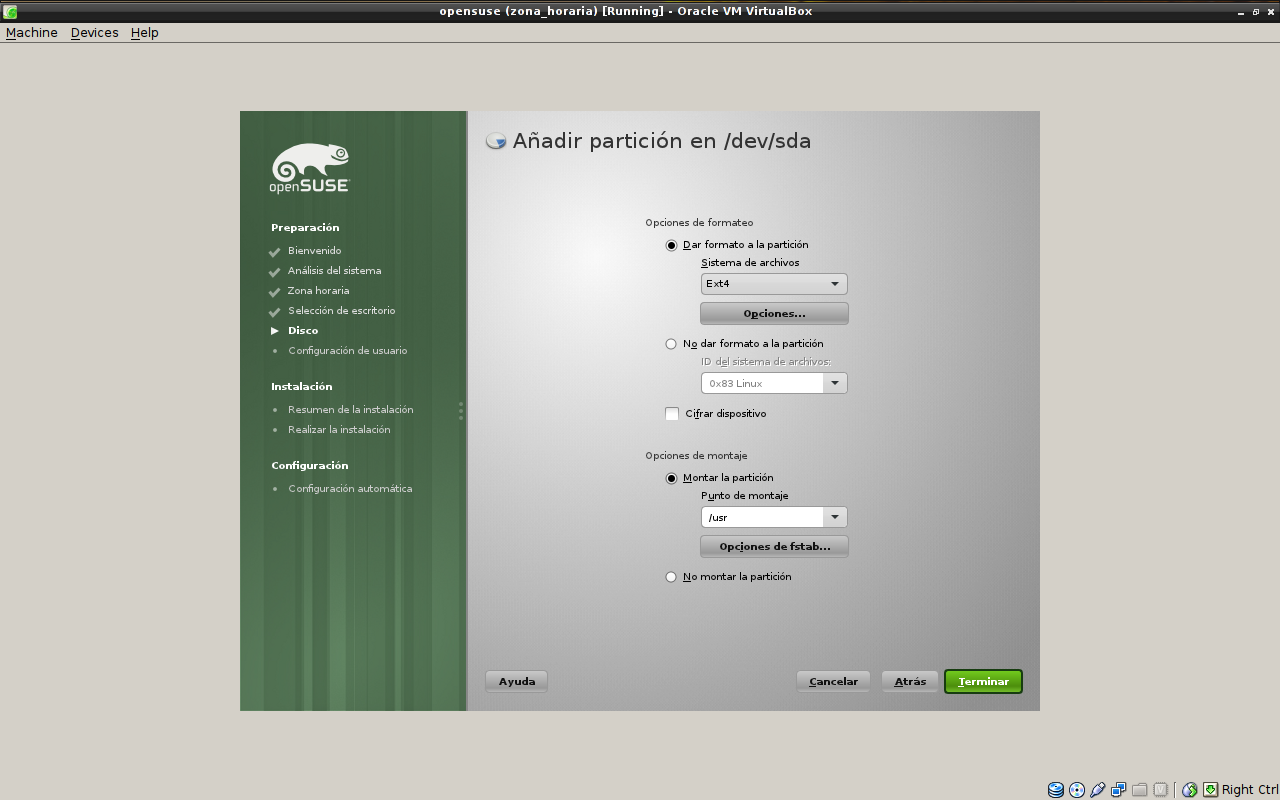
\includegraphics[height=0.8\textheight]{9.png} \hspace*{7.3cm}
\end{frame} 
%%%%%%%%%%%%%%%%%%%%%%%%%%%%%%%%%%%%%%%%%%%%%%%%%%%%%%%%%%%%%%%%%%%%%%%%%%

\begin{frame}
\frametitle{La Instalaci\'on}
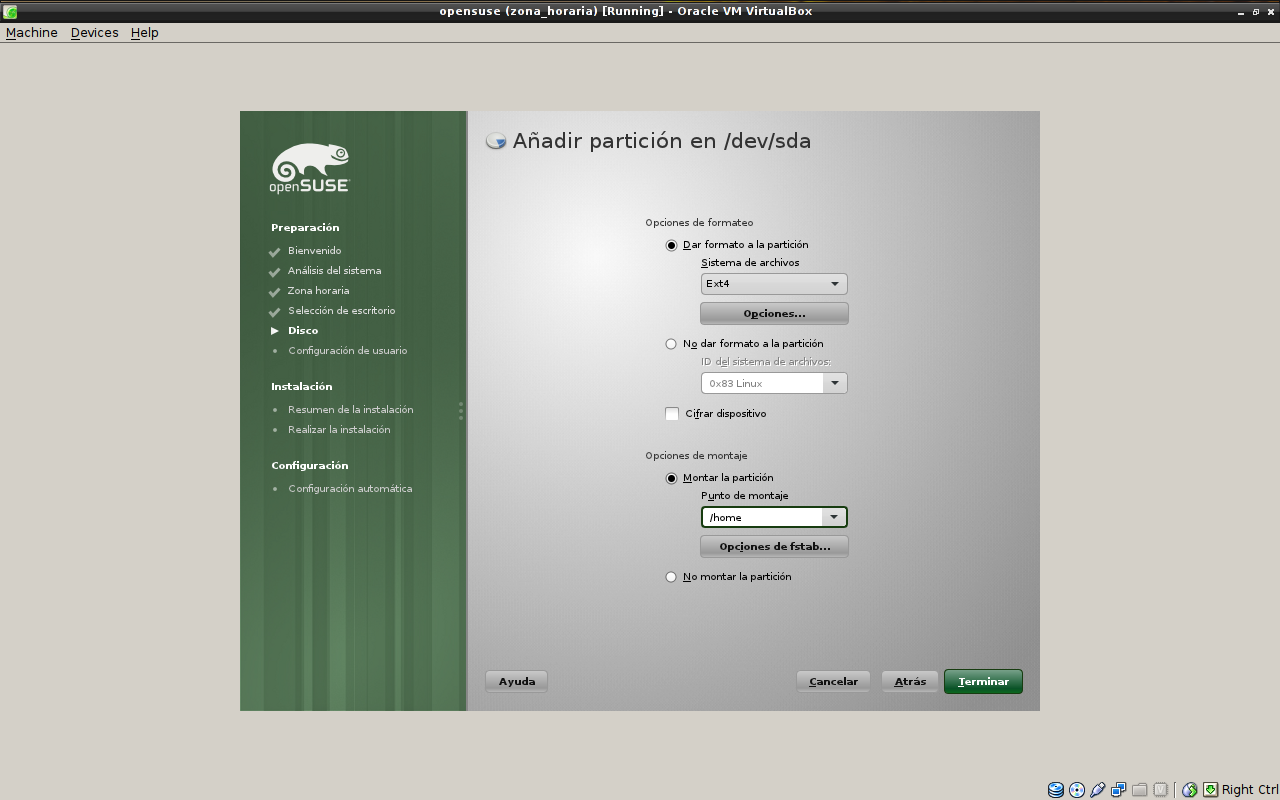
\includegraphics[height=0.8\textheight]{10.png} \hspace*{7.3cm}
\end{frame} 
%%%%%%%%%%%%%%%%%%%%%%%%%%%%%%%%%%%%%%%%%%%%%%%%%%%%%%%%%%%%%%%%%%%%%%%%%%

\begin{frame}
\frametitle{La Instalaci\'on}
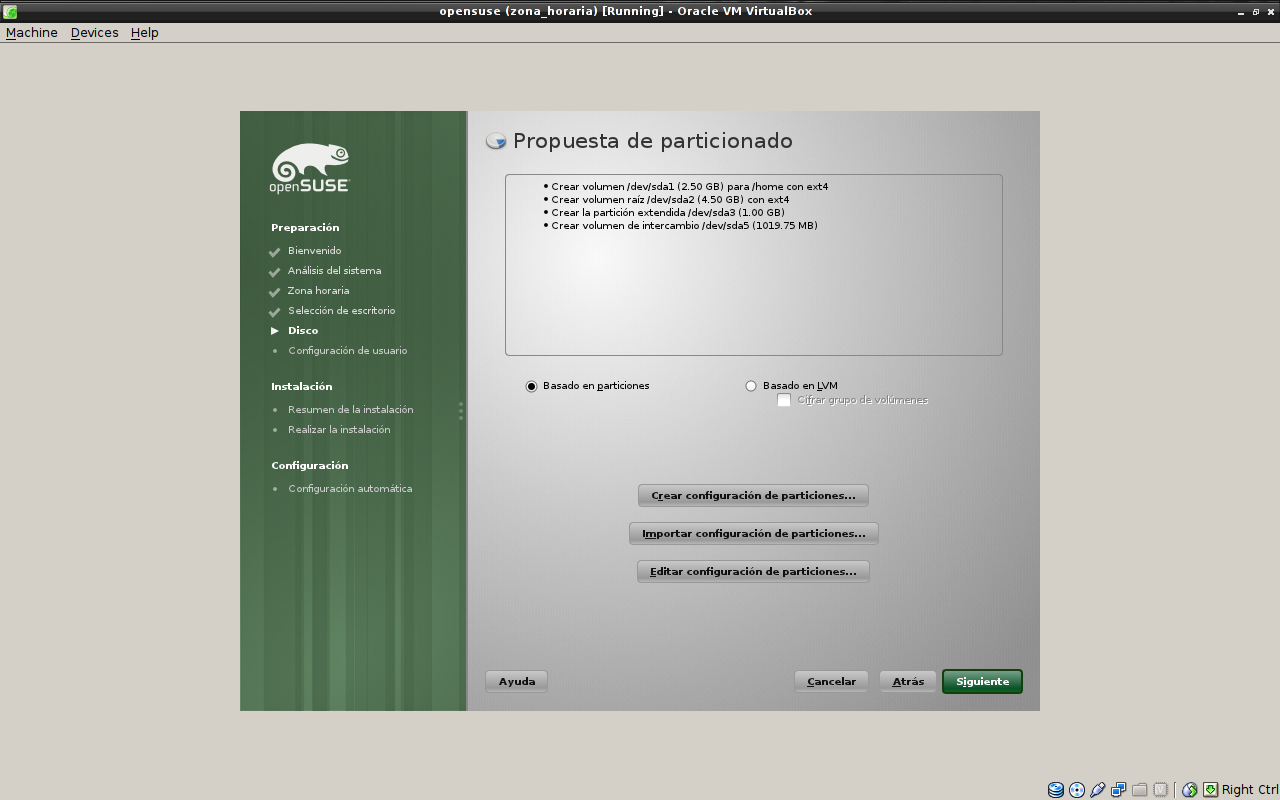
\includegraphics[height=0.8\textheight]{11.png} \hspace*{7.3cm}
\end{frame} 
%%%%%%%%%%%%%%%%%%%%%%%%%%%%%%%%%%%%%%%%%%%%%%%%%%%%%%%%%%%%%%%%%%%%%%%%%%

\begin{frame}
\frametitle{La Instalaci\'on}
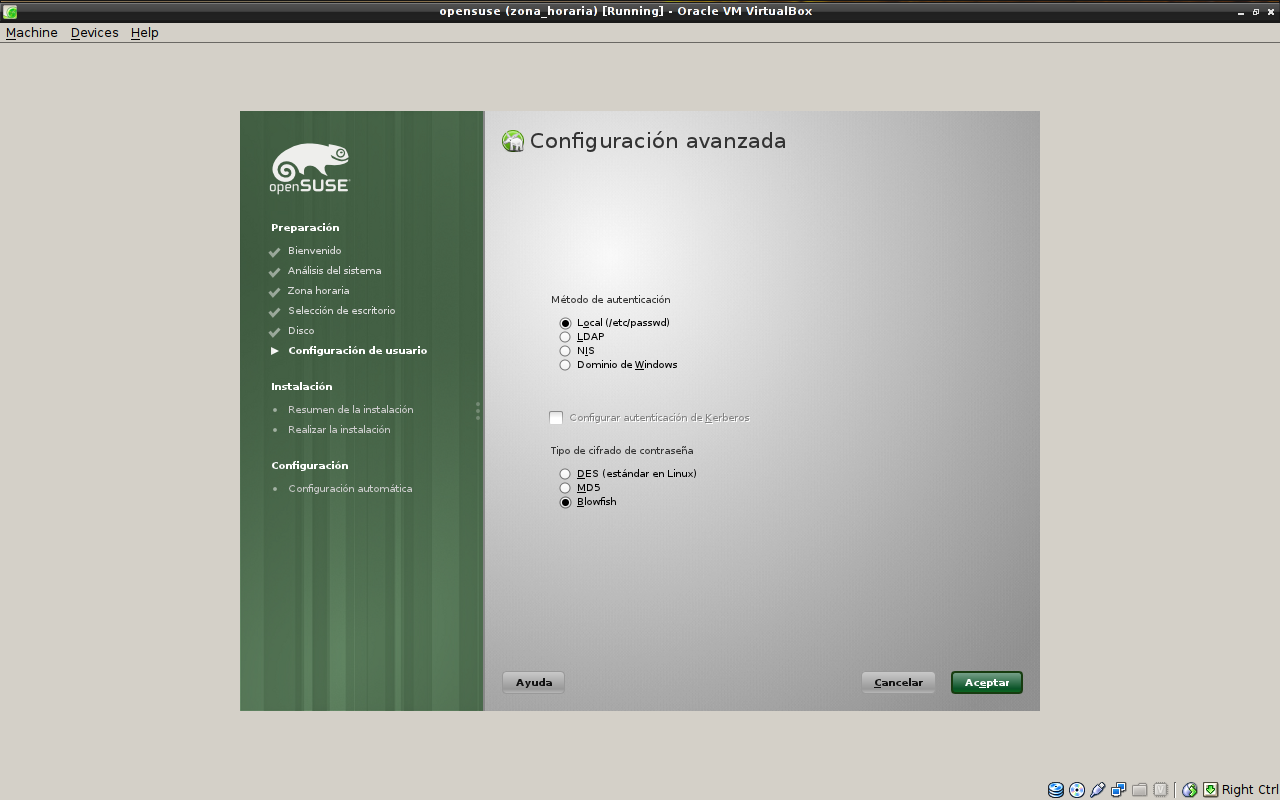
\includegraphics[height=0.8\textheight]{12.png} \hspace*{7.3cm}
\end{frame} 
%%%%%%%%%%%%%%%%%%%%%%%%%%%%%%%%%%%%%%%%%%%%%%%%%%%%%%%%%%%%%%%%%%%%%%%%%%

\begin{frame}
\frametitle{La Instalaci\'on}
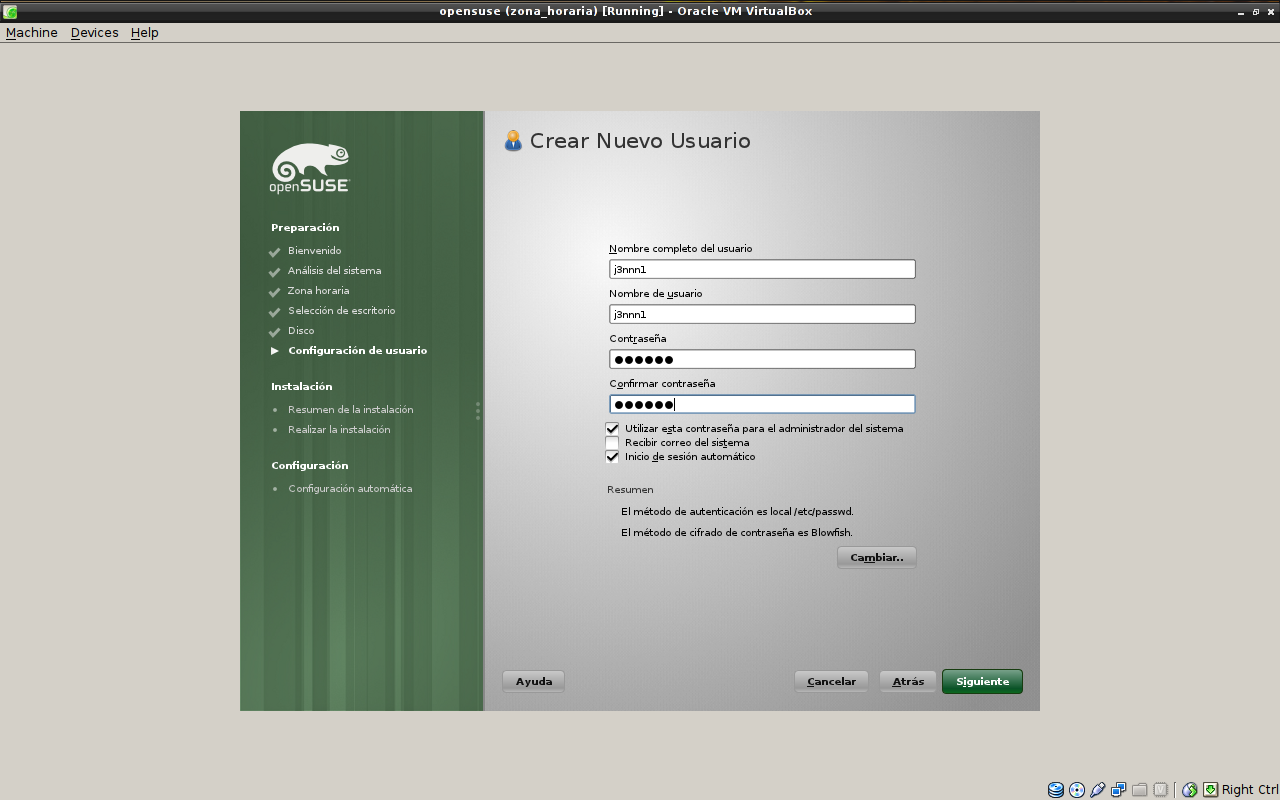
\includegraphics[height=0.8\textheight]{12_.png} \hspace*{7.3cm}
\end{frame} 
%%%%%%%%%%%%%%%%%%%%%%%%%%%%%%%%%%%%%%%%%%%%%%%%%%%%%%%%%%%%%%%%%%%%%%%%%%
\begin{frame}
\frametitle{La Instalaci\'on}
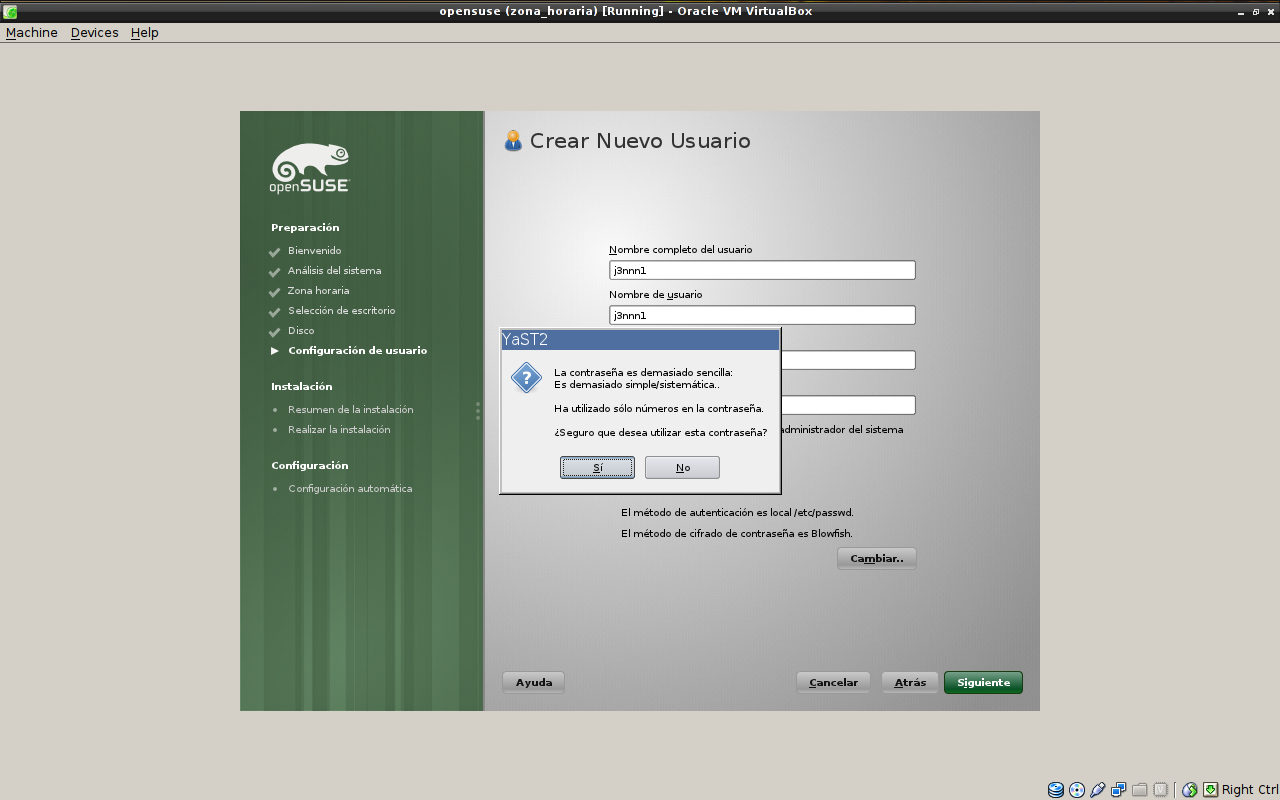
\includegraphics[height=0.8\textheight]{13.png} \hspace*{7.3cm}
\end{frame} 
%%%%%%%%%%%%%%%%%%%%%%%%%%%%%%%%%%%%%%%%%%%%%%%%%%%%%%%%%%%%%%%%%%%%%%%%%%

\begin{frame}
\frametitle{La Instalaci\'on}
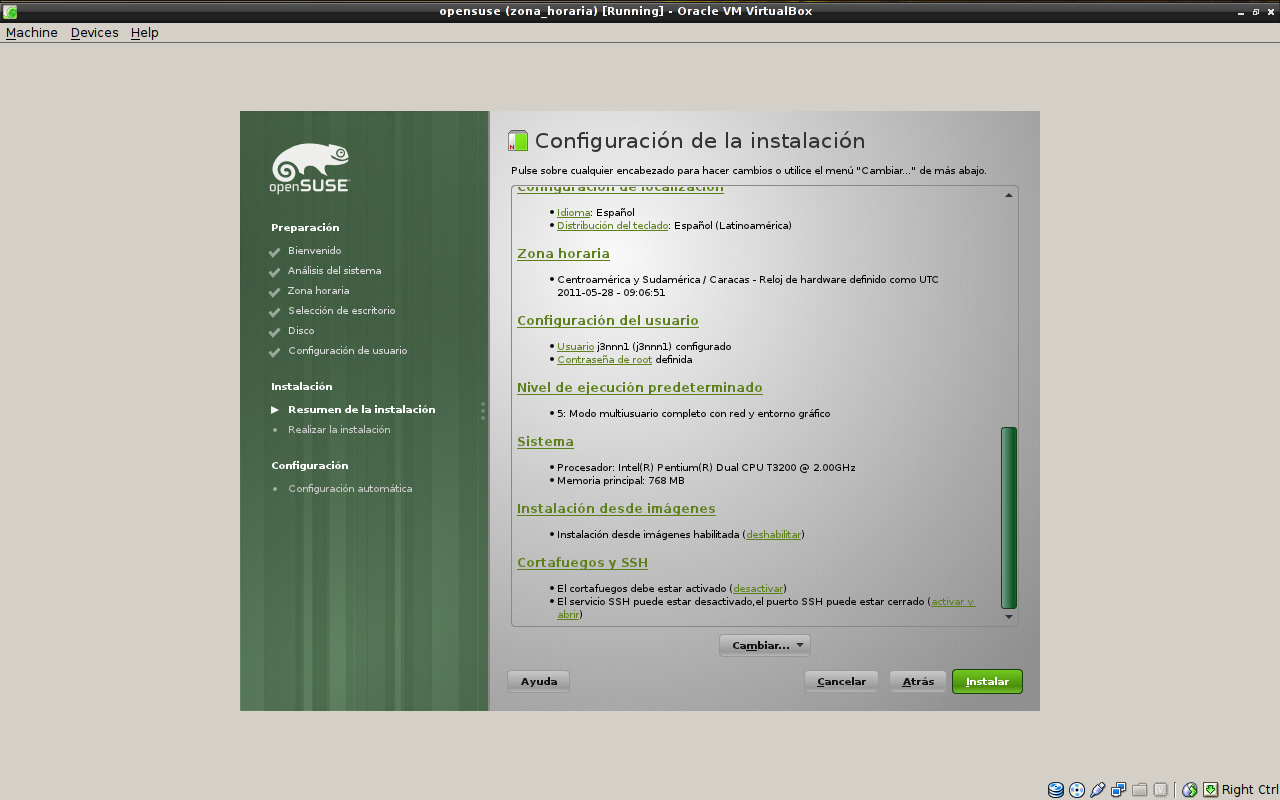
\includegraphics[height=0.8\textheight]{14_.png} \hspace*{7.3cm}
\end{frame} 
%%%%%%%%%%%%%%%%%%%%%%%%%%%%%%%%%%%%%%%%%%%%%%%%%%%%%%%%%%%%%%%%%%%%%%%%%%

\begin{frame}
\frametitle{La Instalaci\'on}
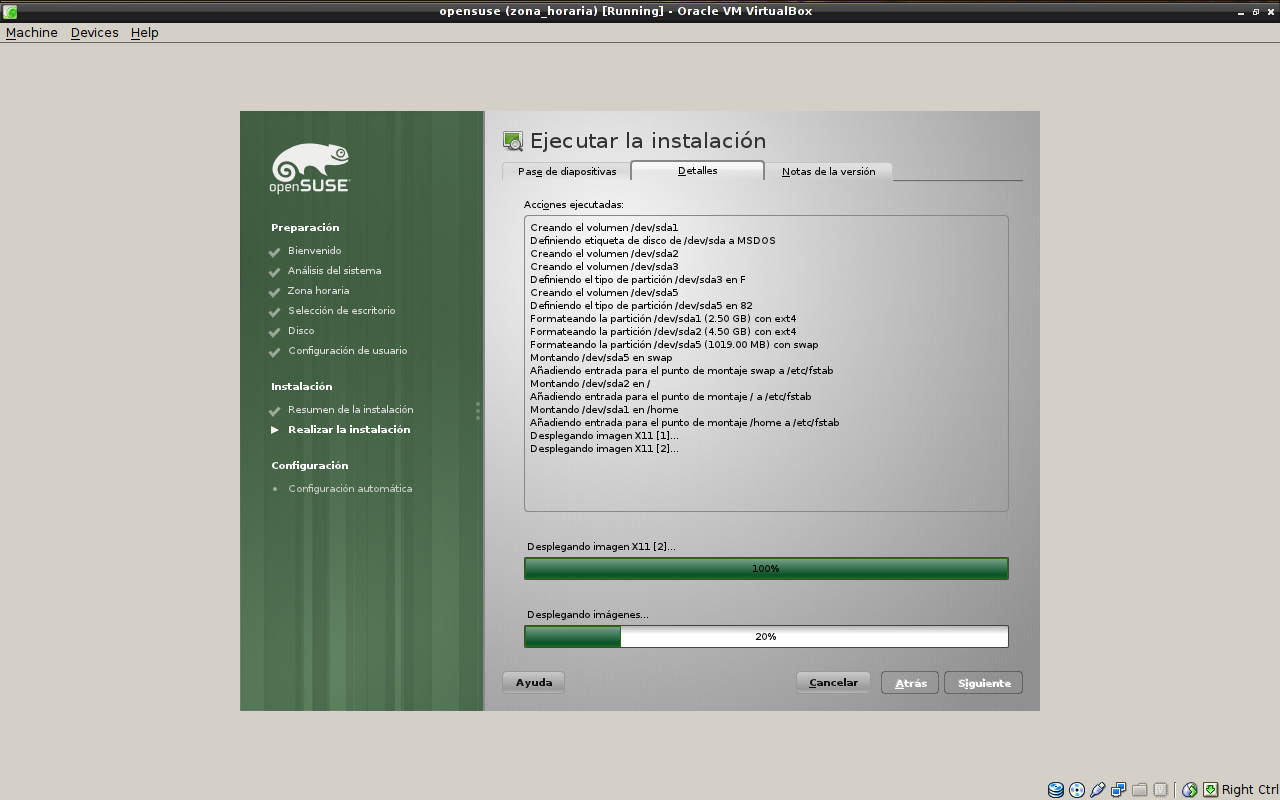
\includegraphics[height=0.8\textheight]{16_.png} \hspace*{7.3cm}
\end{frame} 
%%%%%%%%%%%%%%%%%%%%%%%%%%%%%%%%%%%%%%%%%%%%%%%%%%%%%%%%%%%%%%%%%%%%%%%%%%
\begin{frame}
\frametitle{La Instalaci\'on}
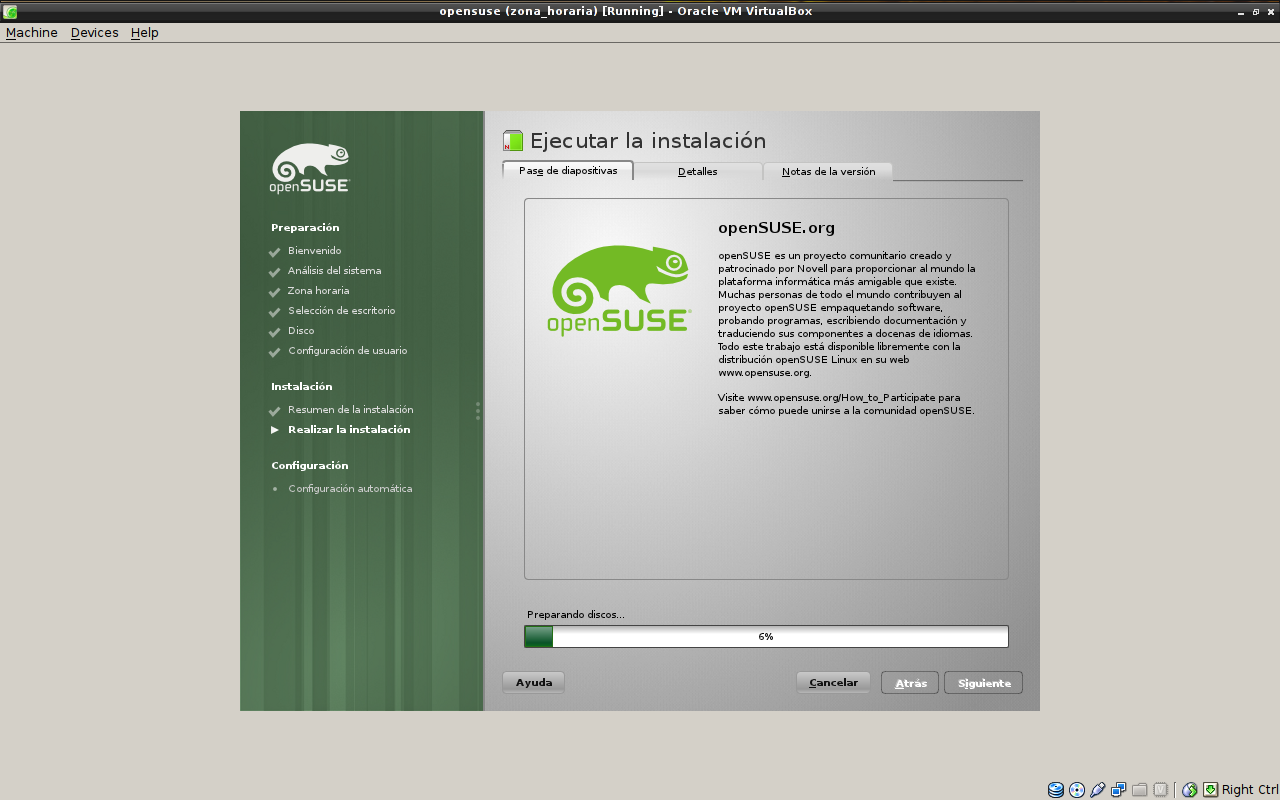
\includegraphics[height=0.8\textheight]{17_.png} \hspace*{7.3cm}
\end{frame} 
%%%%%%%%%%%%%%%%%%%%%%%%%%%%%%%%%%%%%%%%%%%%%%%%%%%%%%%%%%%%%%%%%%%%%%%%%%

\begin{frame}
\frametitle{La Instalaci\'on}
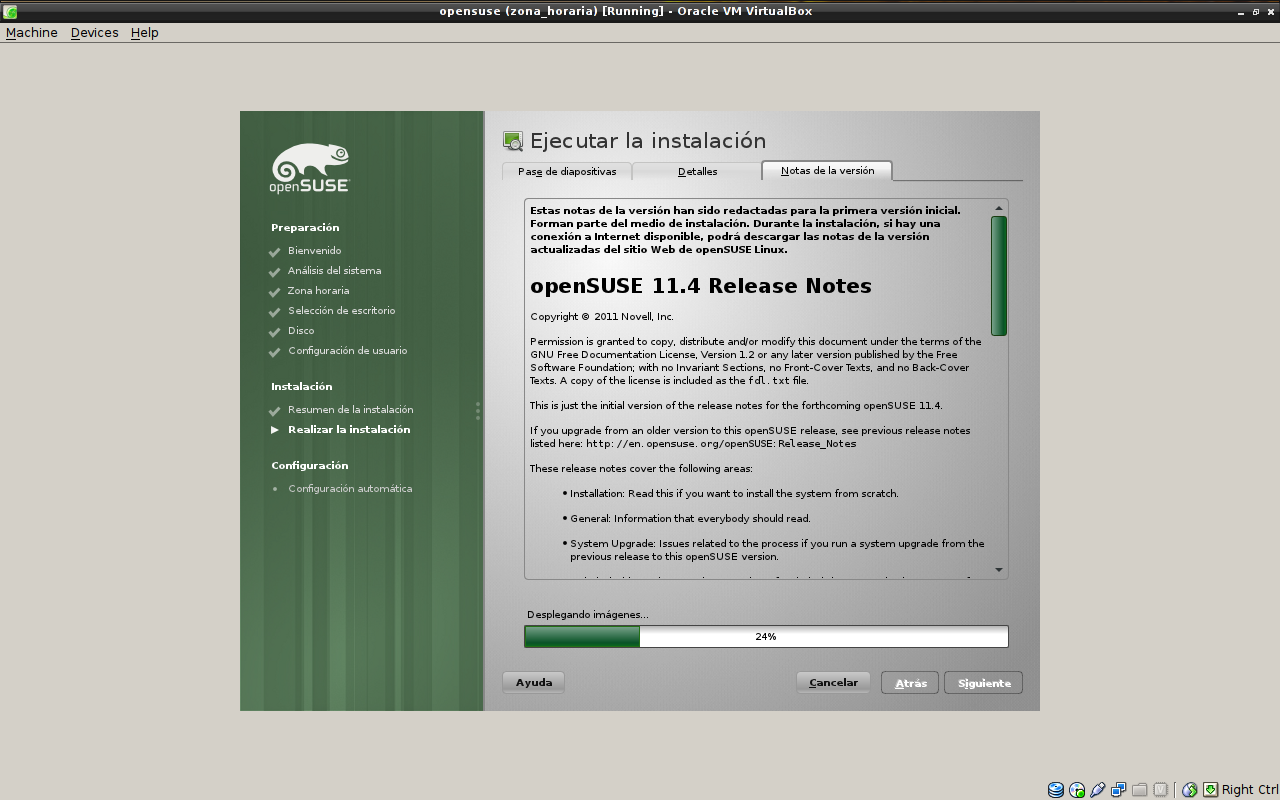
\includegraphics[height=0.8\textheight]{18_.png} \hspace*{7.3cm}
\end{frame} 
%%%%%%%%%%%%%%%%%%%%%%%%%%%%%%%%%%%%%%%%%%%%%%%%%%%%%%%%%%%%%%%%%%%%%%%%%%

\begin{frame}
\frametitle{La Instalaci\'on}
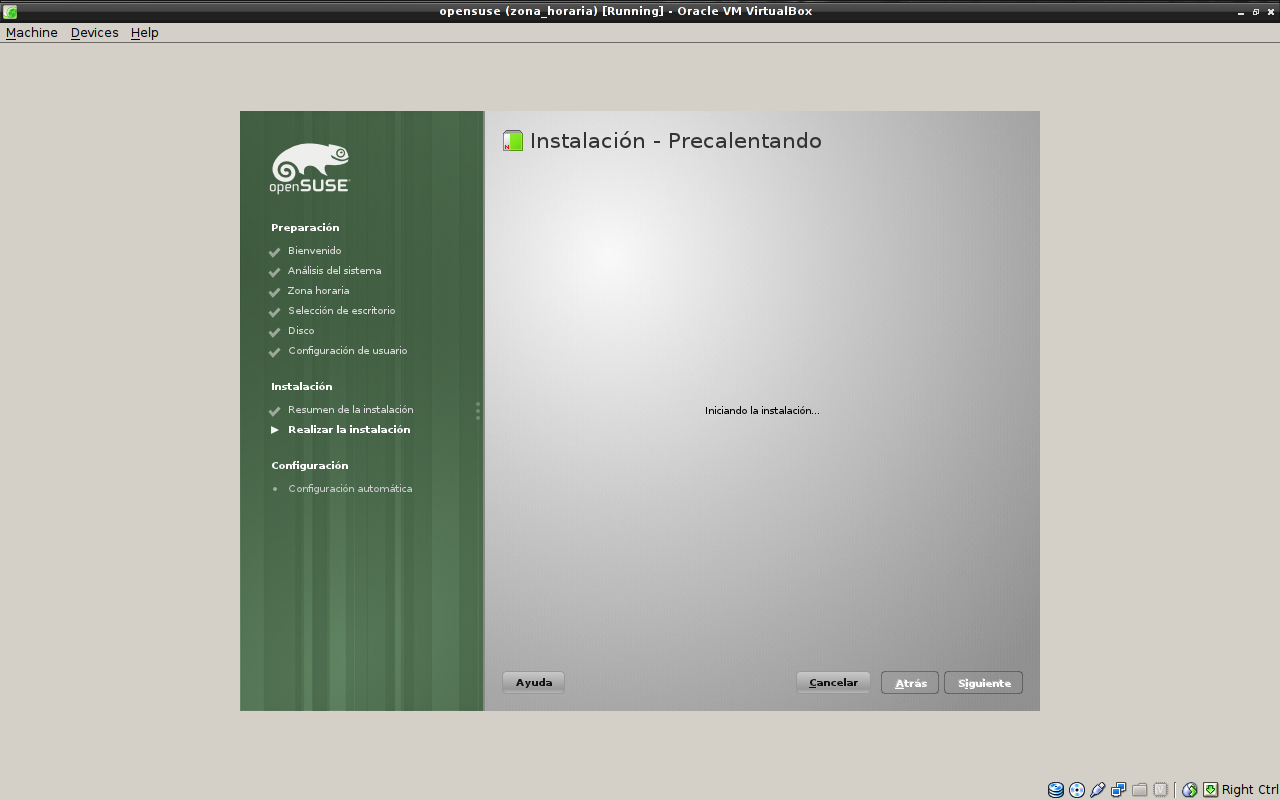
\includegraphics[height=0.8\textheight]{19.png} \hspace*{7.3cm}
\end{frame} 
%%%%%%%%%%%%%%%%%%%%%%%%%%%%%%%%%%%%%%%%%%%%%%%%%%%%%%%%%%%%%%%%%%%%%%%%%%

\begin{frame}
\frametitle{La Instalaci\'on}
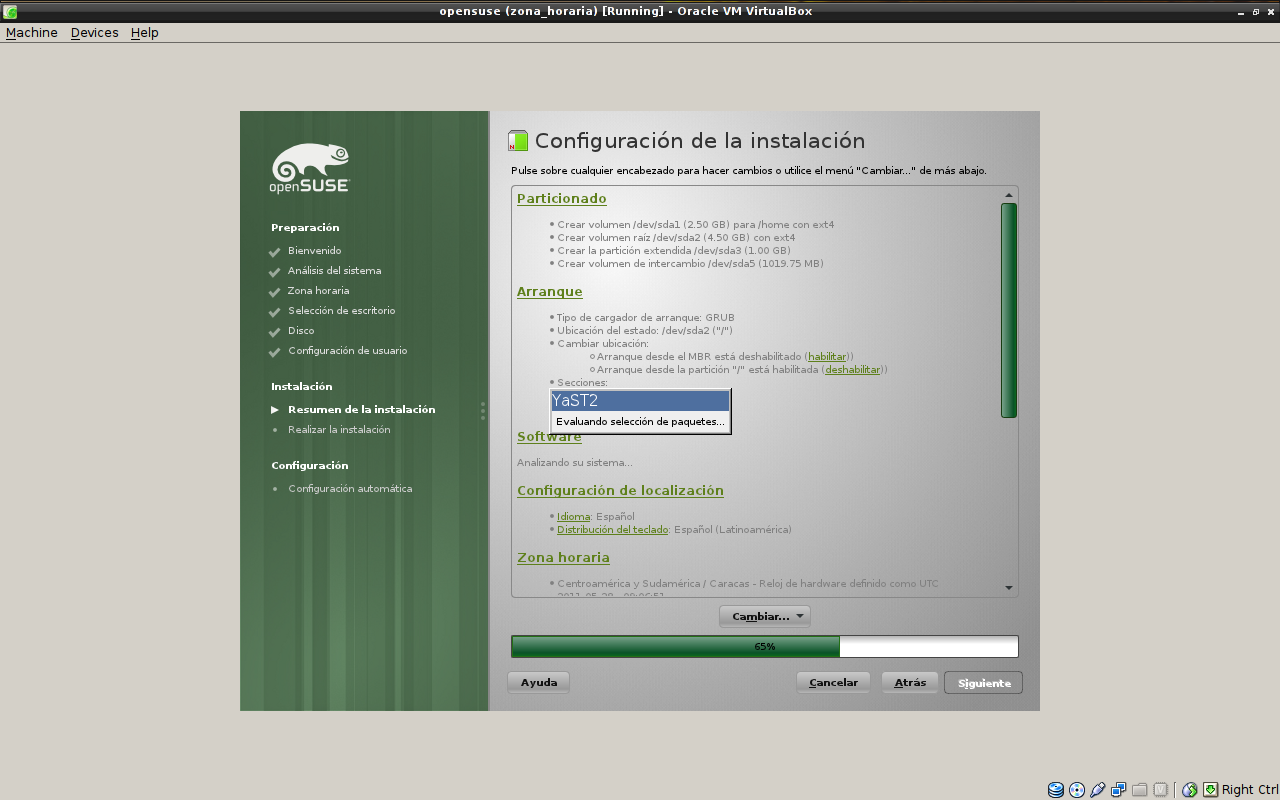
\includegraphics[height=0.8\textheight]{20.png} \hspace*{7.3cm}
\end{frame} 
%%%%%%%%%%%%%%%%%%%%%%%%%%%%%%%%%%%%%%%%%%%%%%%%%%%%%%%%%%%%%%%%%%%%%%%%%%

\section{Configuraciones Generales de Escritorio}
\subsection{Menu Sistema}
\begin{frame}
\frametitle{El Escritorio}
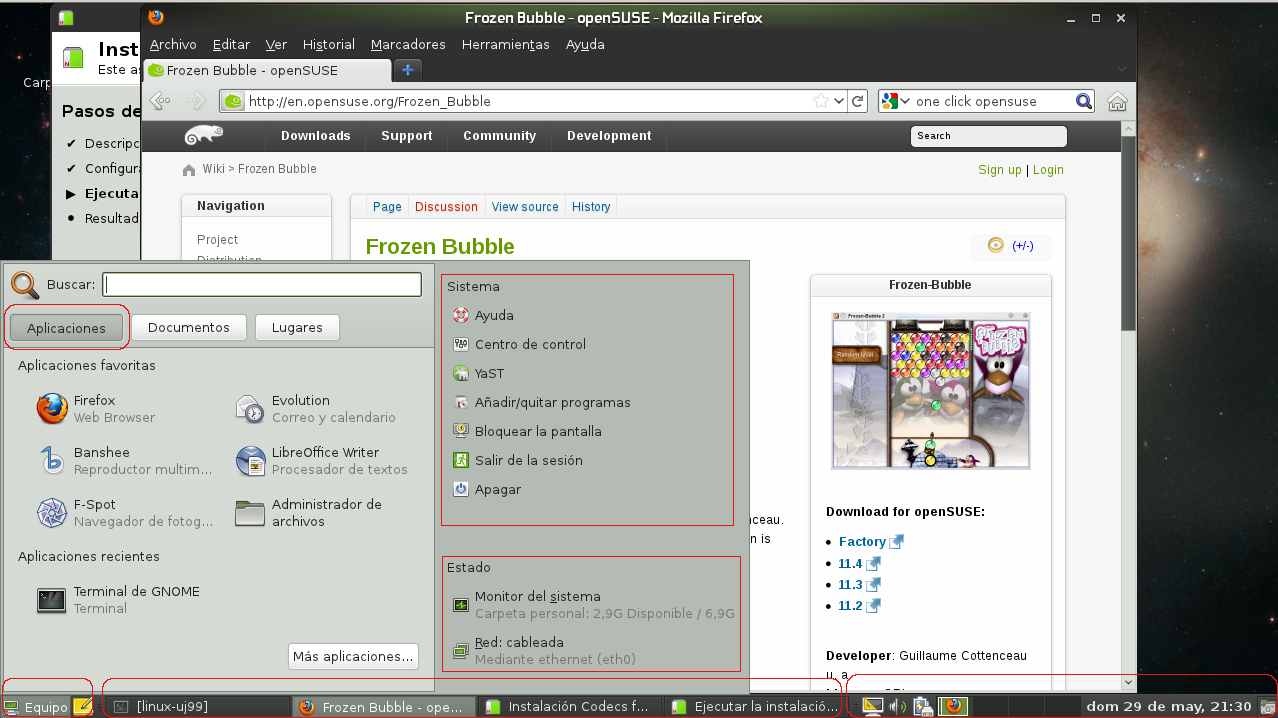
\includegraphics[height=0.8\textheight]{desktop1.png} \hspace*{7.3cm}
\end{frame} 
%%%%%%%%%%%%%%%%%%%%%%%%%%%%%%%%%%%%%%%%%%%%%%%%%%%%%%%%%%%%%%%%%%%%%%%%%%

\subsection{Menu Aplicaciones}
\begin{frame}
\frametitle{El Escritorio}
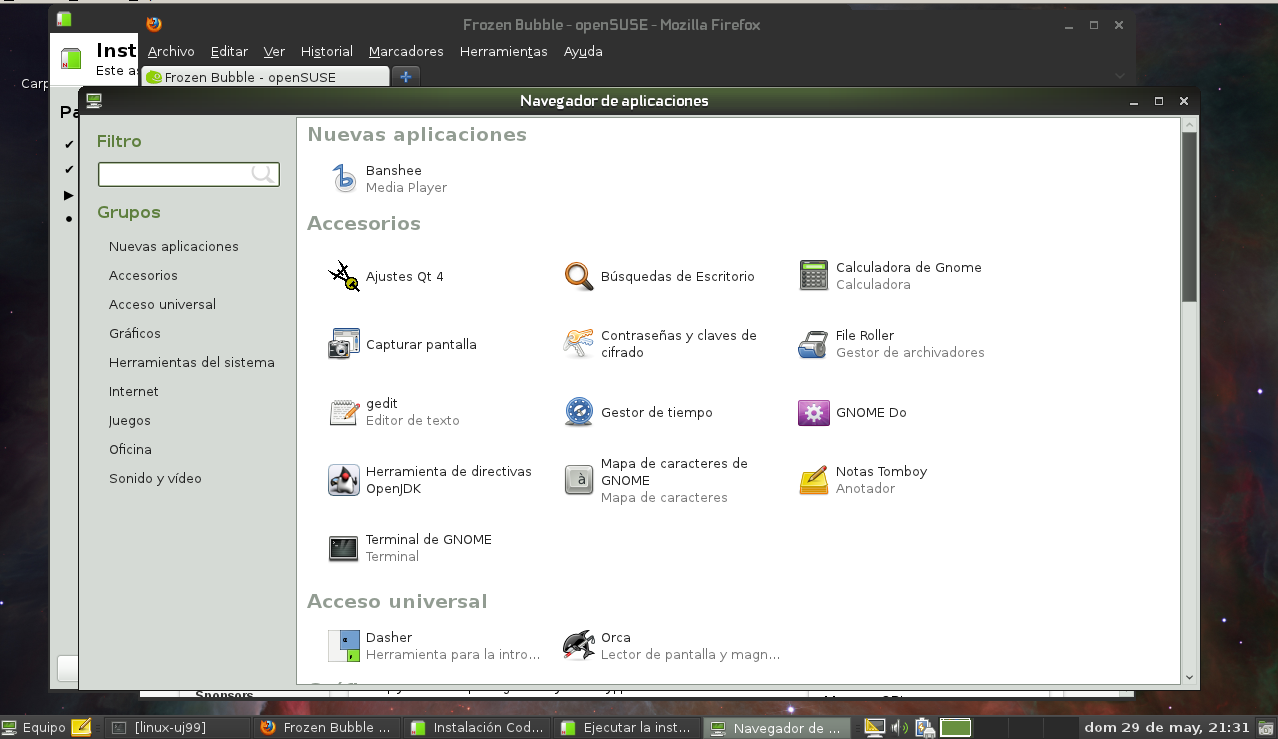
\includegraphics[height=0.8\textheight]{desktop2.png} \hspace*{7.3cm}
\end{frame} 
%%%%%%%%%%%%%%%%%%%%%%%%%%%%%%%%%%%%%%%%%%%%%%%%%%%%%%%%%%%%%%%%%%%%%%%%%%

\subsection{Menu Lugares}
\begin{frame}
\frametitle{El Escritorio}
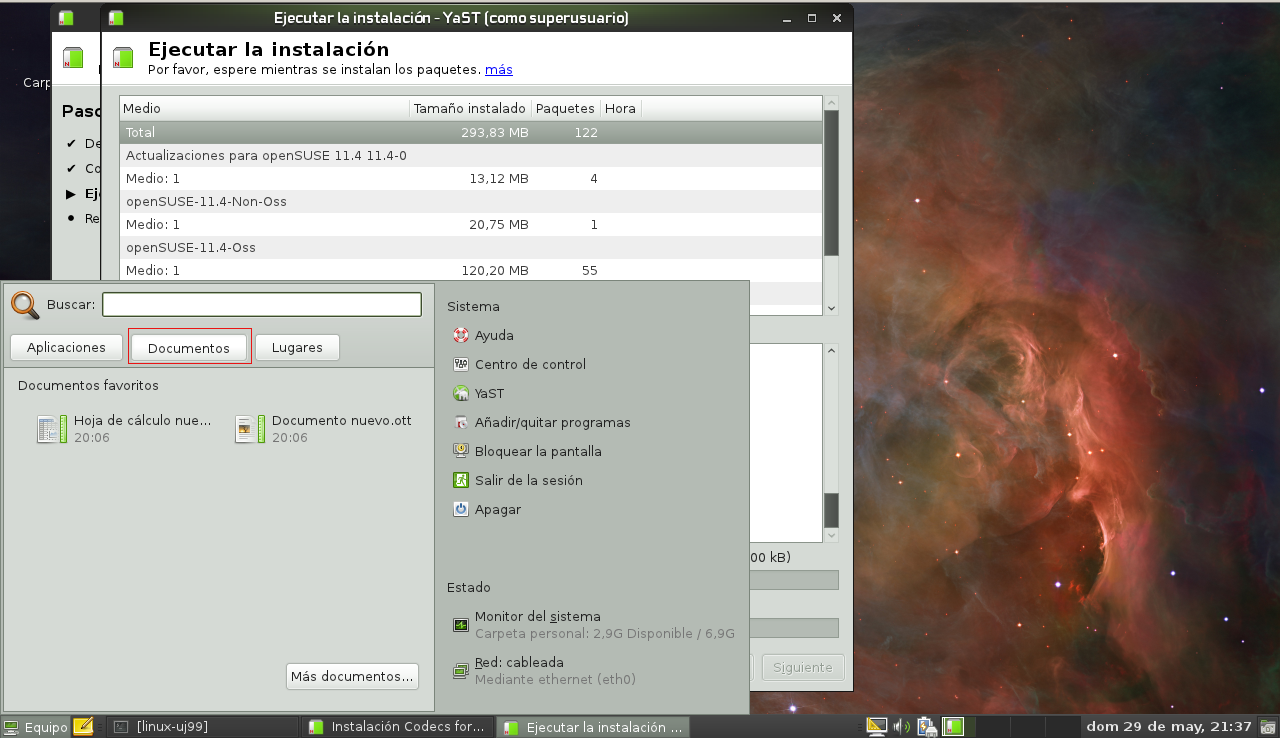
\includegraphics[height=0.8\textheight]{desktop3.png} \hspace*{7.3cm}
\end{frame} 
%%%%%%%%%%%%%%%%%%%%%%%%%%%%%%%%%%%%%%%%%%%%%%%%%%%%%%%%%%%%%%%%%%%%%%%%%%

\subsection{Efectos Especiales}
\begin{frame}
\frametitle{El Escritorio}
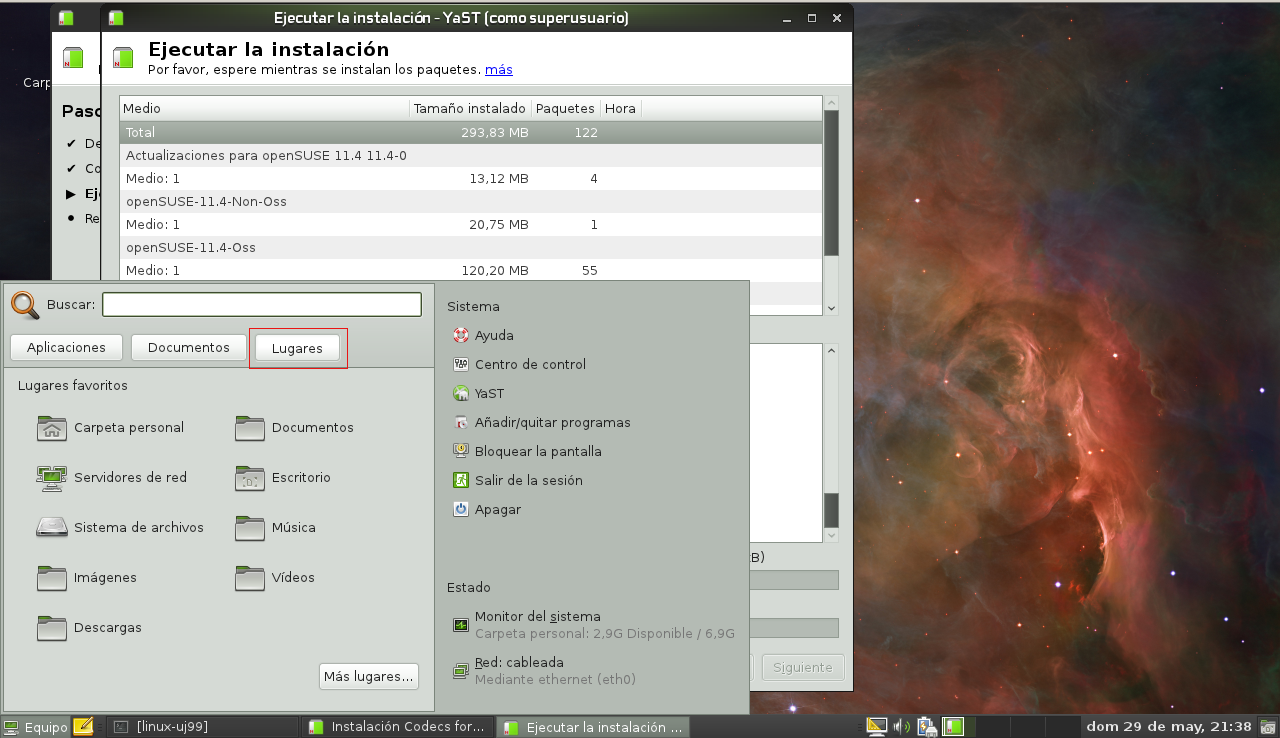
\includegraphics[height=0.8\textheight]{desktop4.png} \hspace*{7.3cm}
\end{frame} 
%%%%%%%%%%%%%%%%%%%%%%%%%%%%%%%%%%%%%%%%%%%%%%%%%%%%%%%%%%%%%%%%%%%%%%%%%%

\section{Agregar o Quitar Programas}
\subsection{Herramientas gr\'aficas}
\begin{frame}
\tableofcontents[currentsection]
\frametitle{Herramientas gr\'aficas}
\end{frame} 
%%%%%%%%%%%%%%%%%%%%%%%%%%%%%%%%%%%%%%%%%%%%%%%%%%%%%%%%%%%%%%%%%%%%%%%%%%

\begin{frame}
\frametitle{Herramientas gr\'aficas}
\begin{itemize}
\item Yast2 o Yast (Yet another setup tool): Es un Manejador de Paquetes
\item Instalaci\'on de 1 click, en p\'aginas que direccionan a un archivo con extensi\'on .ypm, a través de botones como el siguiente:
\item colecci\'on de un click:  http://opensuse-community.org/1-click-collection

\includegraphics[height=0.1\textheight]{boton.png} \hspace*{7.3cm}
\end{itemize}
\end{frame} 
%%%%%%%%%%%%%%%%%%%%%%%%%%%%%%%%%%%%%%%%%%%%%%%%%%%%%%%%%%%%%%%%%%%%%%%%%%


\begin{frame}
  \frametitle{Yast2}
  \begin{columns}
  \column{.5\linewidth}
			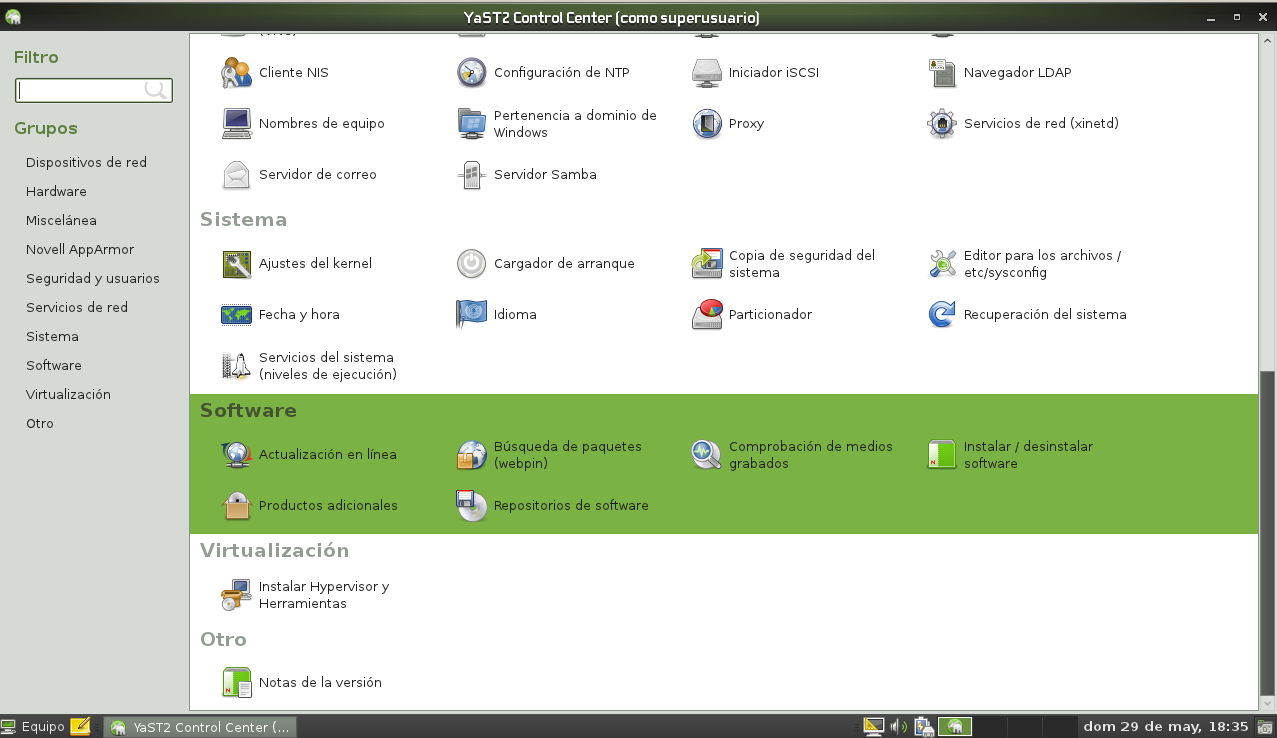
\includegraphics[ width=0.9\textwidth]{instpaquete.png} 
  \column{.5\linewidth}
			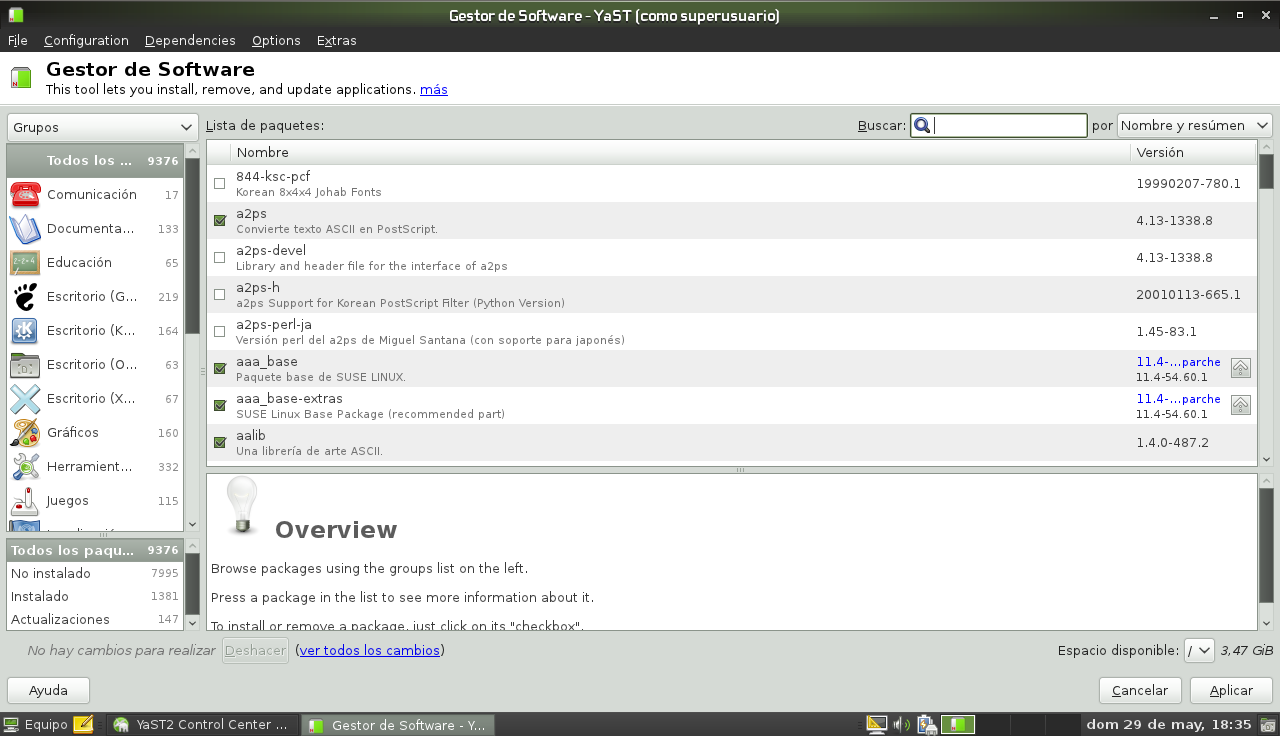
\includegraphics[ width=0.9\textwidth]{yast2.png} 
  \end{columns}
\end{frame}
%%%%%%%%%%%%%%%%%%%%%%%%%%%%%%%%%%%%%%%%%%%%%%%%%%%%%%%%%%%%%%%%%%%%%%%%%%

\subsection{Herramientas NO gr\'aficas}
\begin{frame}
\frametitle{Herramientas No gr\'aficas}
	\begin{itemize}
	\item Instalar nuevos programas.
		\begin{itemize}
			\item \alert{zypper search  NombrePaquete}
			\item \alert{zypper install NombrePaquete.rpm}
			\item \alert{zypper install NombrePaquete}
			\item \alert{zypper ps}
			\item  rpm -qa |grep -i paquete-a-buscar
			\item  rpm -i skype.rpm o NombrePaquete
			\item OCICLI http://opensuse-community.org/nvidia.ymp
			\item yast -i skype-2.2.0.25-suse.i586.rpm
			\item A trav\'es de la fuente tarball tar.gz
		\end{itemize}
	\item Desintalar programas.
		\begin{itemize}
			\item zypper remove NombrePaquete
			\item zypper remove NombrePaquete.rpm
			\item rpm -e VMware-workstation 
		\end{itemize}
	\end{itemize}
\end{frame} 
%%%%%%%%%%%%%%%%%%%%%%%%%%%%%%%%%%%%%%%%%%%%%%%%%%%%%%%%%%%%%%%%%%%%%%%%%%

\begin{frame}
\begin{itemize}
\item Actualizaciones y Parches de seguridad.
	\begin{itemize}
		\item zipper update
                \item zipper patch
        \end{itemize}
\item Administrando repositorios.
        \begin{itemize}
                \item zypper addrepo -f http://ftp.gwdg.de/pub/linux/packman/suse/11.4/ packman
                \item zypper modifyrepo -d Packman
                \item zypper removerepo http://ftp.gwdg.de/pub/linux/packman/suse/11.4
                \item zypper repos -d
                \item zypper addrepo --help
        \end{itemize}
\end{itemize}
\end{frame}
%%%%%%%%%%%%%%%%%%%%%%%%%%%%%%%%%%%%%%%%%%%%%%%%%%%%%%%%%%%%%%%%%%%%%%%%%%

\section{Tareas Administrativas.}
\begin{frame}
\tableofcontents[currentsection]
\frametitle{Tareas Administrativas}
\end{frame} 

\subsection{Administraci\'on de usuarios}
\begin{frame}
\frametitle{A\~nadiendo usuarios}
\begin{itemize}
\item useradd (En Debian y Ubuntu, existe adduser)
\item userdel
\item usermod
\item whoami
\item who
\item id
\end{itemize}
\end{frame}
%%%%%%%%%%%%%%%%%%%%%%%%%%%%%%%%%%%%%%%%%%%%%%%%%%%%%%%%%%%%%%%%%%%%%%%%%%

\subsection{Administraci\'on de usuarios}
\begin{frame}
\frametitle{Usuarios y grupos}
	\begin{itemize}
	\item gpasswd -a usuario grupo
	\item gpasswd -d usuario grupo
	\item groupadd grupo
	\item groupdel grupo
	\item groupmod admin -m newmember
	\item chgrp [-R] grupo archivo
	\item chown [-R] usuario archivo / chown [-R] usuario:grupo archivo
	\end{itemize}
\end{frame}
%%%%%%%%%%%%%%%%%%%%%%%%%%%%%%%%%%%%%%%%%%%%%%%%%%%%%%%%%%%%%%%%%%%%%%%%%%

\subsection{Administraci\'on de usuarios}
\begin{frame}
\frametitle{Usuarios y grupos}
\begin{itemize}
\item /etc/passwd
\item /etc/shadow 
\item /etc/group
\item /etc/skel
\end{itemize}
\end{frame}
%%%%%%%%%%%%%%%%%%%%%%%%%%%%%%%%%%%%%%%%%%%%%%%%%%%%%%%%%%%%%%%%%%%%%%%%%%

\subsection{Administraci\'on de usuarios}
\begin{frame}
\frametitle{Usuarios y grupos}
\begin{itemize}
	\item Estructura del Archivo /etc/passwd.
		\begin{itemize}
		\item Login del usuario.
		\item x si existe password en el /etc/shadow.
		\item UID
		\item GID
		\item GECOS, (General Comprehensive Operating System \'o General Electric Comprehensive Operating Supervisor) 
		\item directorio HOME
		\item Shell de inicio
		\end{itemize}
\end{itemize}
\end{frame}
%%%%%%%%%%%%%%%%%%%%%%%%%%%%%%%%%%%%%%%%%%%%%%%%%%%%%%%%%%%%%%%%%%%%%%%%%%

\subsection{Administraci\'on de usuarios}
\begin{frame}
\begin{itemize}
\item Estructura del Archivo /etc/shadow
	\begin{itemize}
	\item Login del usuario
	\item password encriptado
	\item d\'ias transucrrido desde 1970 del \'ultimo cambio de password.
	\item M\'inimo de d\'ias antes que el password pueda ser cambiado.
	\item M\'aximo de d\'ias para cambiar el password.
	\item D\'ias de advertencias antes de que el password expire.
	\item D\'ias despues de expirado un password cuando la cuenta sea deshabilitada.
	\item D\'ias transcurridos desde 1-1-1970 en que ha estado deshabilitada.
	\item Reservado por sistema 
	\end{itemize}
\end{itemize}
\end{frame}
%%%%%%%%%%%%%%%%%%%%%%%%%%%%%%%%%%%%%%%%%%%%%%%%%%%%%%%%%%%%%%%%%%%%%%%%%%

\subsection{Permisolog\'ia en los archivos}
\begin{frame}
\frametitle{Permisolog\'ia en los archivos}
	\begin{itemize}
	\item S\'olo el propietario del archivo puede cambiar su permiso de acceso.
	\item chmod
	\item c\'alculo de forma octal para representar con bits los permisos
		\begin{itemize}
			\item Debemos saber el valor de bits para cada acci\'on, lectura 4 escritura 2 ejecuci\'on 1
			\item el primer valor es para el usuario due\~no del archivo, el segundo valor es para el grupo, y el tercer valor para otros.
			\item \alert {Ejemplo: } chmod 777 archivo, chmod 644 archivo, chmod 755 archivo, chmod 751 archivo
		\end{itemize}
	\end{itemize}
\end{frame}
%%%%%%%%%%%%%%%%%%%%%%%%%%%%%%%%%%%%%%%%%%%%%%%%%%%%%%%%%%%%%%%%%%%%%%%%%%

\begin{frame}
\begin{itemize}
\frametitle{Permisolog\'ia en los archivos}
\item Mediante comandos simb\'olico o  letras
\begin{itemize}
\item r (lectura), w (escritura), x (ejecuci\'on)
\item u (usuario), g (grupo) ,o (otros)
\item + (a\~nadir),  - (eliminar),  = (mantener)
\item \alert{Ejemplo:} chmod [ugo] [+-=] [rwx] Archivo.txt
\item chmod uog-xw+r permiso.txt, chmod +x archivo.txt
\end{itemize}
\end{itemize}
\end{frame}
%%%%%%%%%%%%%%%%%%%%%%%%%%%%%%%%%%%%%%%%%%%%%%%%%%%%%%%%%%%%%%%%%%%%%%%%%%

\begin{frame}
\frametitle{Permisos de Directorios}
\begin{itemize}
\item r puede leer la lista de directorios (no implica que se pueda acceder a los archivos)
\item w puede escribir en el directorio (crear, renombrar y borrar archivos)
\item x puede buscar en el directorio (entrar y acceder a los archivos)
	\begin{itemize}
	\item para leer, escribir, y crear un archivo, el directorio debe tener el permiso de ejecuci\'on x
	\end{itemize}
\end{itemize}
\end{frame}
%%%%%%%%%%%%%%%%%%%%%%%%%%%%%%%%%%%%%%%%%%%%%%%%%%%%%%%%%%%%%%%%%%%%%%%%%%
%%umask
\subsection{Ambiente y variables de entorno}
\begin{frame}
	\frametitle{Ambiente y variables de entorno}
	\begin{itemize}
		\item Archivos importantes de configuraci\'on en las variables de entorno
		\item Variables de entorno en el ámbito de una terminal.
			\begin{itemize}
			\item /etc/profile
			\item /etc/bash\_bashrc
			\item ~/bash.bashrc
			\end{itemize}
		\item Variables de entorno que afectan a todo el sistema y no se encuentran atadas a una terminal
			\begin{itemize}
			\item /etc/enviroment
			\end{itemize}
	\end{itemize}
\end{frame} 
%%%%%%%%%%%%%%%%%%%%%%%%%%%%%%%%%%%%%%%%%%%%%%%%%%%%%%%%%%%%%%%%%%%%%%%%%%

\subsection{Ambiente y variables de entorno}
\begin{frame}
	\begin{itemize}
		\item PATH contiene los directorios en los cuales se encuentran los binarios.
		\item HOME ruta de la carpeta de archivos personales.
		\item DISPLAY contiene el identificador del display que los programas del servidor X deben usar por defecto.
		\item RANDOM, arroja un numero pseudo aleatorio, cada vez que se utiliza.
		\item LANG, contiene el locale (juego de caracteres que caracterizan un idioma o localidad) por defecto del sistema, tiene relacion LC\_ALL  ignorar el contenido de la variable LANG.
	\end{itemize}
\end{frame} 
%%%%%%%%%%%%%%%%%%%%%%%%%%%%%%%%%%%%%%%%%%%%%%%%%%%%%%%%%%%%%%%%%%%%%%%%%%

\begin{frame}
	\begin{itemize}
		\item LC\_COLLATE : Controla la forma de clasificar: que letras van antes y despu\'es de otras en orden alfab\'etico.
		\item LC\_CTYPE: Controla la correspondencia entre letras may\'usculas y min\'usculas adem\'as de definir los componentes de las diferentes clases de caracteres, como los caracteres alfanum\'ericos. 
		\item SHELL imprime el tipo de shell que se est\'a usando. HISTFILE, nombre del archivo donde se almacenaran los comandos ejecutados.
		\item USER, USERNAME, imprime el nombre del usuario. HOSTNAME, nombre del sistema.
		\item OSTYPE, tipo de sistema operativo ejecutandose. HTTP\_PROXY, indica la ip, o nombre del servidor proxy.
		\item comandos para manejo del entornos de variables:
		\begin{itemize}
		\item set ,env,  export, unset
		\item Ejemplo:  export VARIABLE=VALOR, set VARIABLE=VALOR, unset VARIABLE.
		\end{itemize}
	\end{itemize}
\end{frame}
%%%%%%%%%%%%%%%%%%%%%%%%%%%%%%%%%%%%%%%%%%%%%%%%%%%%%%%%%%%%%%%%%%%%%%%%%%

\subsection{Archivos de bit\'acoras}
\begin{frame}
\frametitle{Archivos de Bit\'acora}
\begin{itemize}
\item /var/log/Xorg.0.log
\item /var/log/zypper.log 
\item /var/log/messages
\item /var/log/lastlog
\item /var/log/firewall
\item /var/log/mail
\item /var/log/pm-powersave.log
\item /var/adm/syslog.log \'o /var/log/syslog.log
\end{itemize}
\end{frame} 
%%%%%%%%%%%%%%%%%%%%%%%%%%%%%%%%%%%%%%%%%%%%%%%%%%%%%%%%%%%%%%%%%%%%%%%%%%


\section{Shell}
\begin{frame}
\frametitle{ Shell }
\begin{definition}
Es una interfaz (CLI, interfaz de l\'inea de comando) que nos proporciona utilidades de trabajo y permite establecer una relaci\'on con el n\'ucleo.
\end{definition}
\end{frame} 
%%%%%%%%%%%%%%%%%%%%%%%%%%%%%%%%%%%%%%%%%%%%%%%%%%%%%%%%%%%%%%%%%%%%%%%%%%

\subsection{Tipos de Shell}
\begin{frame}
\frametitle{ Tipos de Shell }
	\begin{itemize}
		\item Tipo Bourne
		\begin{itemize}
			\item sh
			\item dash reemplazo moderno de ash en Debian
			\item ksh korn shell
			\item zsh Z shell
		\end{itemize}
		\item Tipo consola C
		\begin{itemize}
			\item csh, C shell
			\item tcsh Tenex c shell
		\end{itemize}
	\end{itemize}
\end{frame}
%%%%%%%%%%%%%%%%%%%%%%%%%%%%%%%%%%%%%%%%%%%%%%%%%%%%%%%%%%%%%%%%%%%%%%%%%%

\subsection{Tipos de Shell}
\begin{frame}
\frametitle{Tipo Bourne}
	\begin{itemize}
		\item dash, reemplazo moderno de ash: generalmente en sistemas embebidos, utiliza pocos recursos.
		\item ksh, muchas caracter\'isticas de Cshell, y conjuga caracteristicas de awk, sed, perl en avanzados scripts.
		\item zsh, similar a ksh sin embargo a\~nade más caracter\'isticas de csh. 
	\end{itemize}
\end{frame}
%%%%%%%%%%%%%%%%%%%%%%%%%%%%%%%%%%%%%%%%%%%%%%%%%%%%%%%%%%%%%%%%%%%%%%%%%%

\subsection{Tipos de Shell}
\begin{frame}
\frametitle{Tipo C}
	\begin{itemize}
		\item tcsh,basada en c shell, añade nuevas caracter\'isticas no encontradas en c shell y la puedes encontrar por defecto en sistemas FreeBSD y Darwin.
		\item csh, sintaxis muy similar al lenguaje de programaci\'on C.
	\end{itemize}
\end{frame}
%%%%%%%%%%%%%%%%%%%%%%%%%%%%%%%%%%%%%%%%%%%%%%%%%%%%%%%%%%%%%%%%%%%%%%%%%%

\subsection{Metacaracteres}
\begin{frame}
\frametitle{ Metacaracteres }
	\begin{center}
	\begin{tabular*}{\textwidth}{ @{\extracolsep{\fill}}  | l | c |  }
		\hline
		car\'acter & descripci\'on  \\	
		\hline
		* & {\tiny  uno o m\'as caracteres, es decir a cualquier caracter en nombre de archivo. } \\	
		\hline
		\& & {\tiny Ejecuta un proceso en segundo plano.} \\	
		\hline
		\textgreater \'o \textless \'o \textless \textless \'o \textgreater \textgreater & {\tiny Redirecciona la salida a un archivo.} \\	
		\hline
		\$ & {\tiny Extrae el contenido de una variable.} \\	
		\hline
		\&\&  & {\tiny Condicional AND } \\	
		\hline
		| |  & {\tiny  Condicional OR} \\	
		\hline
	\end{tabular*}
	\end{center}
\end{frame}
%%%%%%%%%%%%%%%%%%%%%%%%%%%%%%%%%%%%%%%%%%%%%%%%%%%%%%%%%%%%%%%%%%%%%%%%%%

\subsection{Metacaracteres}
\begin{frame}
\frametitle{ Metacaracteres }
	\begin{center}
	\begin{tabular*}{\textwidth}{ @{\extracolsep{\fill}}  | l | c | }
		\hline
		car\'acter & descripci\'on  \\	
		\hline
		'[ ]' & {\tiny Denota un rango, '[a-z]' caracteres desde la letra a hasta la z.} \\
		\hline
		! & {\tiny Negaci\'on, '[!a-z]' - Ning\'un caracter que est\'e en el rango desde la a hasta la z.} \\
		\hline
		? & {\tiny cero o un caracter, Equivale a cualquier caracter que aparezca una vez o ninguna. } \\	
		\hline
	\end{tabular*}
	\end{center}
\end{frame}
%%%%%%%%%%%%%%%%%%%%%%%%%%%%%%%%%%%%%%%%%%%%%%%%%%%%%%%%%%%%%%%%%%%%%%%%%%

\subsection{Sentencias y Comandos}
\begin{frame}
\frametitle{Sentencias y Comandos}
\begin{itemize}
\item \alert{Ejecutar comandos}: llamada directa al ejecutable, a trav\'es de una variable de entorno, a trav\'es de un alias.
\item \alert{Separar comandos}: pueden ser separados por (;) , por un backslash ( $\backslash$ ), y colocando cada comando en una l\'inea.
\item \alert{Entrada y Salida Estandar}:
	\begin{itemize}
	\item Entrada Estandar (Teclado), 1 Salida Estandar (Muestra por pantalla ) , 2 Salida de Errores (Salida destinada a los errores o depuraci\'on)
	\item Ejemplo: ls -l | cat \textgreater \textgreater archivo.txt \'o script 2 \textgreater \textgreater archivo.txt \'o   script-programa \textgreater fichero 2\textgreater\&1
	\end{itemize}
\end{itemize}
\end{frame}
%%%%%%%%%%%%%%%%%%%%%%%%%%%%%%%%%%%%%%%%%%%%%%%%%%%%%%%%%%%%%%%%%%%%%%%%%%

\subsection{Utilizado en clase}
\begin{frame}
\frametitle{Buscar informaci\'on en Bit\'acoras}
\begin{itemize}
\item \alert{tail}: tail -f archivo, tail -n30, lista las \'ultimas l\'ineas de un archivo.
\item \alert{head}: head -n40, lista las primeras l\'ineas de un archivo.
\item \alert{cat}: permite combinar o concatenar varios archivos, en caso de un solo archivo muestra todo su contenido.
\item \alert{less}: paginador de textos, q para salir, y con las flechas de navegaci\'on del teclado puedes recorrer el texto.
\item \alert{more}: paginador de textos, q para salir, y con tabulador se desplaza.
\\
\item ls -l | (less/more), tail -n100 | grep "Patr\'onABuscar" | (less/more).
\end{itemize}
\end{frame}
%%%%%%%%%%%%%%%%%%%%%%%%%%%%%%%%%%%%%%%%%%%%%%%%%%%%%%%%%%%%%%%%%%%%%%%%%%

\subsection{Herramientas}
\begin{frame}
\frametitle{Herramientas}
B\'usqueda de informaci\'on:  find, grep, locate, sort, cat, egrep, tail, head, wc, xarg.
Monitoreo de Redes: netstat, traceroute, ping.
Monitoreo local: free, df, last, lastlog, pstree, ps, uptime, top, dmesg. 
Chequeo y Administraci\'on: watch, md5sum, zypper, rpm, diff.
\end{frame}
%%%%%%%%%%%%%%%%%%%%%%%%%%%%%%%%%%%%%%%%%%%%%%%%%%%%%%%%%%%%%%%%%%%%%%%%%%

\subsection{Los Procesos.}
\begin{frame}
\begin{definition}
Es un programa/comando/shellscript que se est\'a ejecutando en memoria, cuando el proceso es finalizado se elimina de memoria. cada proceso tiene un Id que lo identifica como \'unico.
\end{definition}
\end{frame}
%%%%%%%%%%%%%%%%%%%%%%%%%%%%%%%%%%%%%%%%%%%%%%%%%%%%%%%%%%%%%%%%%%%%%%%%%%

\subsection{Tipos de Procesos.}
\begin{frame}
\begin{itemize}
\item Background (Segundo Plano), Procesos iniciados por el sistema, como demonios a trav\'es del  script de arranque por lo general.
\item Foreground (Primer Plano), son procesos iniciados desde una c\'onsola por un usuario, tambi\'en se les dice procesos con contrl de terminal.
\end{itemize}
\end{frame}
%%%%%%%%%%%%%%%%%%%%%%%%%%%%%%%%%%%%%%%%%%%%%%%%%%%%%%%%%%%%%%%%%%%%%%%%%%

\subsection{Los Procesos.}
\begin{frame}
\frametitle{Los Procesos.}
\begin{itemize}
\item Listando procesos: ps aux, a selecciona todos los procesos no asociados a una terminal, u despliega formato orientado al usuario, x procesos asociados a una terminal.
\end{itemize}
\end{frame}
%%%%%%%%%%%%%%%%%%%%%%%%%%%%%%%%%%%%%%%%%%%%%%%%%%%%%%%%%%%%%%%%%%%%%%%%%%

\subsection{Comandos para el Control de Procesos}
\begin{frame}
\frametitle{Comandos para el Control de Procesos.}
\begin{itemize}
\item ps permite desplegar los procesos actuales.
\item pstre muestra el \'arbol de procesos.
\end{itemize}
\end{frame}
%%%%%%%%%%%%%%%%%%%%%%%%%%%%%%%%%%%%%%%%%%%%%%%%%%%%%%%%%%%%%%%%%%%%%%%%%%

\subsection{Comandos para el Control de Procesos}
\begin{frame}
\frametitle{Comandos para el Control de Procesos.}
\begin{itemize}
\item jobs: lista los procesos ejecutandose en background
\item kill: se usa para enviar se\~nales a procesos en ejecuci\'on. Ejemplo: kill \textless se\~nal \textgreater PID, kill -l (lista las se\~nales disponibles), kill -SIGTERM 12345, kill -15 12345.
\item bg, fg: Se usa para enviar procesos detenidos al modo background, y fg se usa prar enviar los procesos ejecut\'andose en background al modo foreground.
\item nice: te permite asignar prioridad a un proceso, antes de ejecutarse. Ejemplo: nice 19 procesoaEjecutar.
\item renice:  te permite modificar el valor de la prioridad a los procesos luego de iniciarlo, o estando en ejecuci\'on. Ejemplo:  renice 18 PID.
\end{itemize}
\end{frame}
%%%%%%%%%%%%%%%%%%%%%%%%%%%%%%%%%%%%%%%%%%%%%%%%%%%%%%%%%%%%%%%%%%%%%%%%%%

\subsection{Utilizando kill}
\begin{frame}
\frametitle{Utilizando kill}
\begin{itemize}
\item kill -9 NROPROCESO
\item kill -SIGTERM NROPROCESO
\item kill -1 NROPROCESO
\item kill -HUP NROPROCESO (Procesos Zombie)
\item kill -15 NROPROCESO (Terminaci\'on de un proceso)
\end{itemize}
\end{frame}
%%%%%%%%%%%%%%%%%%%%%%%%%%%%%%%%%%%%%%%%%%%%%%%%%%%%%%%%%%%%%%%%%%%%%%%%%%

\subsection{Procesos Agradables..}
\begin{frame}
\frametitle{Procesos Agradables..}
\begin{itemize}
\item El valor de nice puede variar de -19 a 19, siendo el m\'as negativo con mayor prioridad (es el m\'as desagradable) a medida que el valor es positivo tiene menor prioridad de procesamiento.
\item Solo puedes modificar la prioridad de procesos si le pertenecen al usuario, a menos que sea root.
\item nice 10 BINARIOAEJECUTAR
\item renice 15 PID (N\'umero de Proceso)
\end{itemize}
\end{frame}
%%%%%%%%%%%%%%%%%%%%%%%%%%%%%%%%%%%%%%%%%%%%%%%%%%%%%%%%%%%%%%%%%%%%%%%%%%

\subsection{ Monitoreo para el control de Proceso.}
\begin{frame}
\frametitle{Monitoreo para el control de Proceso.}
\begin{itemize}
\item top: es un comando c\'iclico que ordena los primeros 20 procesos, htop (interfaz humana).
\item free: permite ver el uso de la memoria f\'isica y compartida.
\item uptime: tiempo transcurrido desde que se inici\'o la computadora. 
\end{itemize}
\end{frame}
%%%%%%%%%%%%%%%%%%%%%%%%%%%%%%%%%%%%%%%%%%%%%%%%%%%%%%%%%%%%%%%%%%%%%%%%%%

\subsection{Agendar Ejecuci\'on de Procesos.}
\begin{frame}
\frametitle{Agendar Ejecuci\'on de Procesos.}
\begin{itemize}
\item Son procesos iniciados por el demonio Cron, pueden ser recurrentes de forma diaria, semanal o mensual, o de una sola ejecuci\'on.
\item Archivos de configuraci'on:
	\begin{itemize}
	\item General /etc/crontab
	\item Por Usuario: /var/spool/cron/tabs/usuario
	\end{itemize}
\end{itemize}
\end{frame}
%%%%%%%%%%%%%%%%%%%%%%%%%%%%%%%%%%%%%%%%%%%%%%%%%%%%%%%%%%%%%%%%%%%%%%%%%%

\subsection{Agendar Ejecuci\'on de Procesos.}
\begin{frame}
\frametitle{Agendar Ejecuci\'on de Procesos.}
\begin{itemize}
\item Estructura del Archivo crontab (crontab -e)
	\begin{itemize}
	\item Minutos (0-59)
	\item Horas (0-23)
	\item D\'ias (1- 31)
	\item Meses (1-12)
	\item Dia-de-Semana (1-7)
	\item usuario de Ejecuci\'on
	\item comando a ejecutar
	\end{itemize}
\item El Entorno de variables en cron es diferente al establecido por /etc/profile, /etc/bash\_bashrc.
\item crontab -l : lista las entradas del crontab
\item crontab -r :elimina el crontab que ya existe.
\end{itemize}
\end{frame}
%%%%%%%%%%%%%%%%%%%%%%%%%%%%%%%%%%%%%%%%%%%%%%%%%%%%%%%%%%%%%%%%%%%%%%%%%%

\subsection{Directorios para Ejecuci\'on periodica.}
\begin{frame}
\frametitle{Directorios para Ejecuci\'on periodica.}
\begin{itemize}
\item /etc/cron.hourly
\item /etc/cron.daily
\item /etc/cron.weekly
\item /etc/cron.montly
\item Ejemplo: 22 4 * * 0 root comand
\end{itemize}
\end{frame}

\subsection{Introducci\'on a los niveles de Ejecuci\'on}
\begin{frame}
\frametitle{Introducci\'on a los niveles de Ejecuci\'on}
\begin{itemize}
\item Al iniciar un SO linux existe una secuencia de arranque, comenzando por la BIOS al verificar los dispositivos, luego la BIOS si existe alg\'un programa instalado en el MBR lo ejecuta, En este caso encontraremos al GRUB, el cual al inicializar nos muestras los diferentes SO disponibles, al seleccionar alguno disponible se monta en /boot, inicializa los dispositivos de memoria, carga controladores, monta el sistema de archivo / en modo lectura, y ejecuta el proceso init (Proceso padre), el proceso init lee el archivo de configuraci\'on /etc/inittab e inicia los script que corresponde al Nivel De Ejecuci\'on.
\item \alert{Niveles de Ejecuci\'on} Es el modo de operaci\'on que implementan los sistemas Operativos basados en el sistema de arranque tipo Unix System V, Se podría definir como un estado en el que una serie de script se deben ejecutar.
\item Para todas las distribuciones los niveles de ejecuci\'on que no var\'ian son: runlevel 0 (Apagar) y runlevel 6 (reiniciar).
\item Opensuse utiliza el nivel de ejecuci\'on 5 por defecto para mostrar su entorno gráfico.
\end{itemize}
\end{frame}
%%%%%%%%%%%%%%%%%%%%%%%%%%%%%%%%%%%%%%%%%%%%%%%%%%%%%%%%%%%%%%%%%%%%%%%%%%

\subsection{Niveles de Ejecuci\'on}
\begin{frame}
\frametitle{Niveles de Ejecuci\'on}
\begin{itemize}
\item \alert{1}: Modo monousuario, permite hacer reparaciones en el sistema, no ejecuta demonios, ni configura la interfaz de red.
\item \alert{2}: Local multiuser without remote network, multiusuario sin configurar la interfaz de red. 
\item \alert{3}: Full multiuser with network, Multiusuario con acceso a red, sin interfaz gr\'afica.
\item \alert{4}: Not usado por opensuse
\item \alert{5}: Multiusuario con acceso a red, y con interfaz gr\'afica.
\item \alert{6}: Ejecuto los scripts de parada e inicio, para reiniciar el sistema.
\item \alert{0}: Ejecuta los scripts para el cierre del sistema.
\end{itemize}
\end{frame}
%%%%%%%%%%%%%%%%%%%%%%%%%%%%%%%%%%%%%%%%%%%%%%%%%%%%%%%%%%%%%%%%%%%%%%%%%%

\subsection{Introducci\'on a los niveles de Ejecuci\'on}
\begin{frame}
\frametitle{Introducci\'on a los niveles de Ejecuci\'on}
\begin{itemize}
\item Los scripts en opensuse se encuentran en /etc/init.d/rc{0-6}
\item En el directorio anterior se encuentran enlaces simb\'olicos
\item Los scripts en estos directorios tienen una nomeclatura muy particular: EOrdenNombre, donde E puede ser una letra S (start, iniciar proceso) o  K (terminar proceso), Orden es el n\'umero de secuencia(orden de ejecuci\'on), y Nombre es el nombre del script de ejecuci\'on en el directorio /etc/init.d/rc{0-6}.d
\item comandos utilizados para el control de los niveles de ejecuci\'on: runlevel, init, telinit, shutdown, halt, reboot, chkconfig
\item chkconfig -level 345 mysql off|on
\item Menú gráfico en Yast, en la sección de system services.
\end{itemize}
\end{frame}
%%%%%%%%%%%%%%%%%%%%%%%%%%%%%%%%%%%%%%%%%%%%%%%%%%%%%%%%%%%%%%%%%%%%%%%%%%

\subsection{Parada  e inicio de Servicios.}
\begin{frame}
\frametitle{Parada  e inicio de Servicios.}
\begin{itemize}
\item Servicios de Red
\begin{itemize}
\item /etc/services
\item /etc/inetd.conf
\end{itemize}
\item Iniciar un servicio
\begin{itemize}
\item /etc/init.d/servicio restart | stop | start 
\end{itemize}
\item Ver nivel de ejecuci\'on actual: runlevel
\end{itemize}
\end{frame}
%%%%%%%%%%%%%%%%%%%%%%%%%%%%%%%%%%%%%%%%%%%%%%%%%%%%%%%%%%%%%%%%%%%%%%%%%%

\section{Introducci\'on a CUPS}
\begin{frame}{Servicio de Impresión}
\newtheorem{defi}{{\sc Definición}}
\begin{defi}
Son el conjunto de Servicios y programas para manejar y configurar las clases e impresoras y administrar las colas del sistema.
\end{defi}
\begin{itemize}
	\item Berkley Line Printer Deamon (LPD).
	\item System V Line Printer System.
	\item Common Unix Printer System (CUPS).
\end{itemize}
\end{frame}
%%%%%%%%%%%%%%%%%%%%%%%%%%%%%%%%%%%%%%%%%%%%%%%%%%%%%%%%%%%%%%%%%%%%%%%%%%

\begin{frame}{Características Generales de CUPS}
	\begin{itemize}
		\item Basado en Internet Printing Protocol (IPP)
		\item Permite administrar el sistema de impresión mediante una interfaz web, (http://localhost:631)
		\item Soporta el uso de comandos compatibles con Berkeley y System V.
		\item Soporta el manejo de clases de impresoras.
		\item Soporta filtro para imágenes, archivos PDF y de texto.
	\end{itemize}
\end{frame}
%%%%%%%%%%%%%%%%%%%%%%%%%%%%%%%%%%%%%%%%%%%%%%%%%%%%%%%%%%%%%%%%%%%%%%%%%%

\begin{frame}{Modelo general del CUPS}
\begin{itemize}
	\item Archivos de configuración.
	\item Scheduler (filtros, Backend).
	\item CUPS (comandos Berkeley  y System V)
\end{itemize}

\includegraphics[height=5em,width=20em]{cups.png} \hspace*{7.3cm}
\end{frame}
%%%%%%%%%%%%%%%%%%%%%%%%%%%%%%%%%%%%%%%%%%%%%%%%%%%%%%%%%%%%%%%%%%%%%%%%%%

\begin{frame}{CUPS}

\begin{itemize}
\item Inicio de los servicios.
	\begin{itemize}
		\item /etc/init.d/cups (start|stop|restart)
		\item /usr/sbin/cups (binario de CUPS)
	\end{itemize}
\item Archivos de CUPS.
	\begin{itemize}
		\item /etc/cups
			\begin{itemize}
				\item classes.conf
				\item client.conf	
				\item cups.conf
				\item printer.conf
			\end{itemize}
		\item /var/spool/cups/(Archivos de cola de impresión)
		\item /var/log/cups/(logs del servicio CUPS)
		\item /usr/share/doc/packages/cups/(Documentacion CUPS)
	\end{itemize}
\end{itemize}
\end{frame}
%%%%%%%%%%%%%%%%%%%%%%%%%%%%%%%%%%%%%%%%%%%%%%%%%%%%%%%%%%%%%%%%%%%%%%%%%%

\begin{frame}{Comandos para manejar impresoras.}
\begin{itemize}
\item lpadmin:  permite definir y modificar impresoras.
	\begin{itemize}
		\item -d –p –x :  -d define la impresora por defecto en el sistema, la opción  -p configura el nombre de la impresora o clase. Y la opción –x elimina la impresora o clase configurada.
		\item -E : Encriptación de la comunicación con el servidor.
	\end{itemize}
\end{itemize}
\end{frame}

\begin{frame}
	\begin{itemize}
		\item Opciones –p:
		\begin{itemize}
			\item -c nombreclase, añade una impresora a una clase.
			\item -i excluyente de la opción –p donde se define el driver de la impresora (archivo ppd) y permite definir una interfaz al estilo system V.
			\item -m configura una interfaz de acuerdo al estándar system V, o un archivo ppd de acuerdo al modelo de la impresora. (lpinfo obtienes una lista de driver soportados).
			\item -o job-k-limit=value , job-page-limit=value, job-quota-period=value, job-sheets-default=banner, job-sheets-default=banner,banner, printer-is-shared=true/false.
			\item  -r class
			\item  -u allow:user,user,@group
			\item -P ppd-file
			\item -v "device-uri“  identificador de recursos.. Puede ser un archivo file://recurso, socket://hostname:9100, parallel:/dev/lp1 , http://hostname:631/ipp/ , lpd://hostname/queue, lpd://hostname/queue
		\end{itemize}
	\end{itemize}
\end{frame}
%%%%%%%%%%%%%%%%%%%%%%%%%%%%%%%%%%%%%%%%%%%%%%%%%%%%%%%%%%%%%%%%%%%%%%%%%%

\begin{frame}{Para Ejecutar..}
\begin{itemize}
	\item Lpadmin : lpadmin -p Deskjet -E -v parallel:/dev/lp1  (-m archivo.ppd)
	\item lpinfo –v lista dispositivos disponibles.
	\item lpinfo –m lista drivers disponibles en CUPS.
	\item lpc status
	\item lpadmin -d Deskjet
	\item lp -d Deskjet archivo.txt (opcional –n numero de copias)
	\item Lpq
	\item Lprm 1
	\item Cancel 2
\end{itemize}
\end{frame}
%%%%%%%%%%%%%%%%%%%%%%%%%%%%%%%%%%%%%%%%%%%%%%%%%%%%%%%%%%%%%%%%%%%%%%%%%%

\begin{frame}{Manejar Jobs..}
\begin{itemize}
	\item Imprimir un archivo. 
	\begin{itemize}
		\item Lpr –d impresora archivo (Berkeley system)
		\item Lp –P impresora archivo (system V)
	\end{itemize}
	\item Ver trabajos en la cola de impresión.
	\begin{itemize}
		\item Lpq
	\end{itemize}
	\item Eliminar trabajos de la cola de impresión.
	\begin{itemize}
		\item Lprm jobid (berkeley) 
		\item Cancel jobid (system V)
	\end{itemize}
	\item Status de Impresoras.
	\begin{itemize}
		\item lpc status
	\end{itemize}
	
\end{itemize}
\end{frame}
%%%%%%%%%%%%%%%%%%%%%%%%%%%%%%%%%%%%%%%%%%%%%%%%%%%%%%%%%%%%%%%%%%%%%%%%%%

\begin{frame}{CUPS}
\begin{itemize}
	\item Colas de impresión.
	\begin{itemize}
		\item 	Enable|Disable impresora
	\end{itemize}
	\item Trabajos de Impresión.
	\begin{itemize}
		\item accept|reject impresora
	\end{itemize}
	\item Clases.
	\begin{itemize}
		\item lpadmin –p impresora –c clase (agregar)
		\item lpadmin –p impresora –r clase (retirar)
		\item lpadmin –x clase (elimina)
	\end{itemize}
\end{itemize}
\end{frame}
%%%%%%%%%%%%%%%%%%%%%%%%%%%%%%%%%%%%%%%%%%%%%%%%%%%%%%%%%%%%%%%%%%%%%%%%%%
\end{document}
